\chapter{LHC and the CMS experiment}
\chaptermark{The LHC and the CMS experiment}  
\thispagestyle{plain}  % First page has default style
\pagestyle{chapterpages}
\label{Section:Chapter3}

\minitoc

The physics analyses presented in this thesis are performed using data generated by the \textbf{\ac{LHC}} and collected by the \textbf{\ac{CMS} experiment}. This chapter begins by exploring how the \ac{LHC} accelerates and collides protons up to centre-of-mass energies ($\sqrt{s}$) of $13.6\TeV$. In turn, this creates the extreme but necessary conditions needed to probe Nature at its smallest length scales. The discussion then shifts to the \ac{CMS} detector, a multipurpose apparatus composed of several layers of specialised subdetectors. These intricate systems work in concert to enable the precise reconstruction of particles emerging from proton-proton (pp) collisions at the heart of the detector.

\section{The LHC}
\label{Section:Chapter3_LHC}
The \ac{LHC}~\cite{LHC_1}, situated at the \ac{CERN} near Geneva, Switzerland, is a testament to human scientific achievement. Housed in the same tunnel that previously accommodated the \ac{LEP} collider, the \ac{LHC} was designed to accelerate beams of hadrons and collide them head-on. It was engineered to reach collision energies of up to $\sqrt{s} = 14\TeV$ and to achieve an unprecedented luminosity of $10^{34}\unit{cm}^{-2}\unit{s}^{-1}$. During the 2015–2018 data-taking period, referred to as ``Run 2", each proton beam reached $6.5\TeV$, corresponding to $\sqrt{s}=13\TeV$. After a multi-year shutdown for maintenance and upgrades, the \ac{LHC} resumed operation in 2022 at $6.8\TeV$ per beam (a new collision energy of $\sqrt{s}=13.6\TeV$), running just below its $14\TeV$ design energy. 

Spanning a circumference of $27\unit{km}$, the \ac{LHC} mirrors the basic layout of its predecessor, the \ac{LEP} collider. The experimental landscape is strategically arranged with two general-purpose experiments, ATLAS~\cite{LHC_ATLAS} and \ac{CMS}~\cite{LHC_CMS}, positioned at diametrically opposite points, Points 1 and 5 respectively. The ALICE experiment~\cite{LHC_ALICE} occupies Point 2, while LHCb~\cite{LHC_LCHb} is situated at Point 8. At these critical locations, the circulating beams are precisely focused and brought into collision. A basic schematic of the \ac{LHC} layout, highlighting the eight arc sections, the two circulating beams, and the locations of these experiments, is shown in Fig.~\ref{Figure:Chapter3_LHC_BasicLayout}.

\begin{figure}[!htbp]
\centering
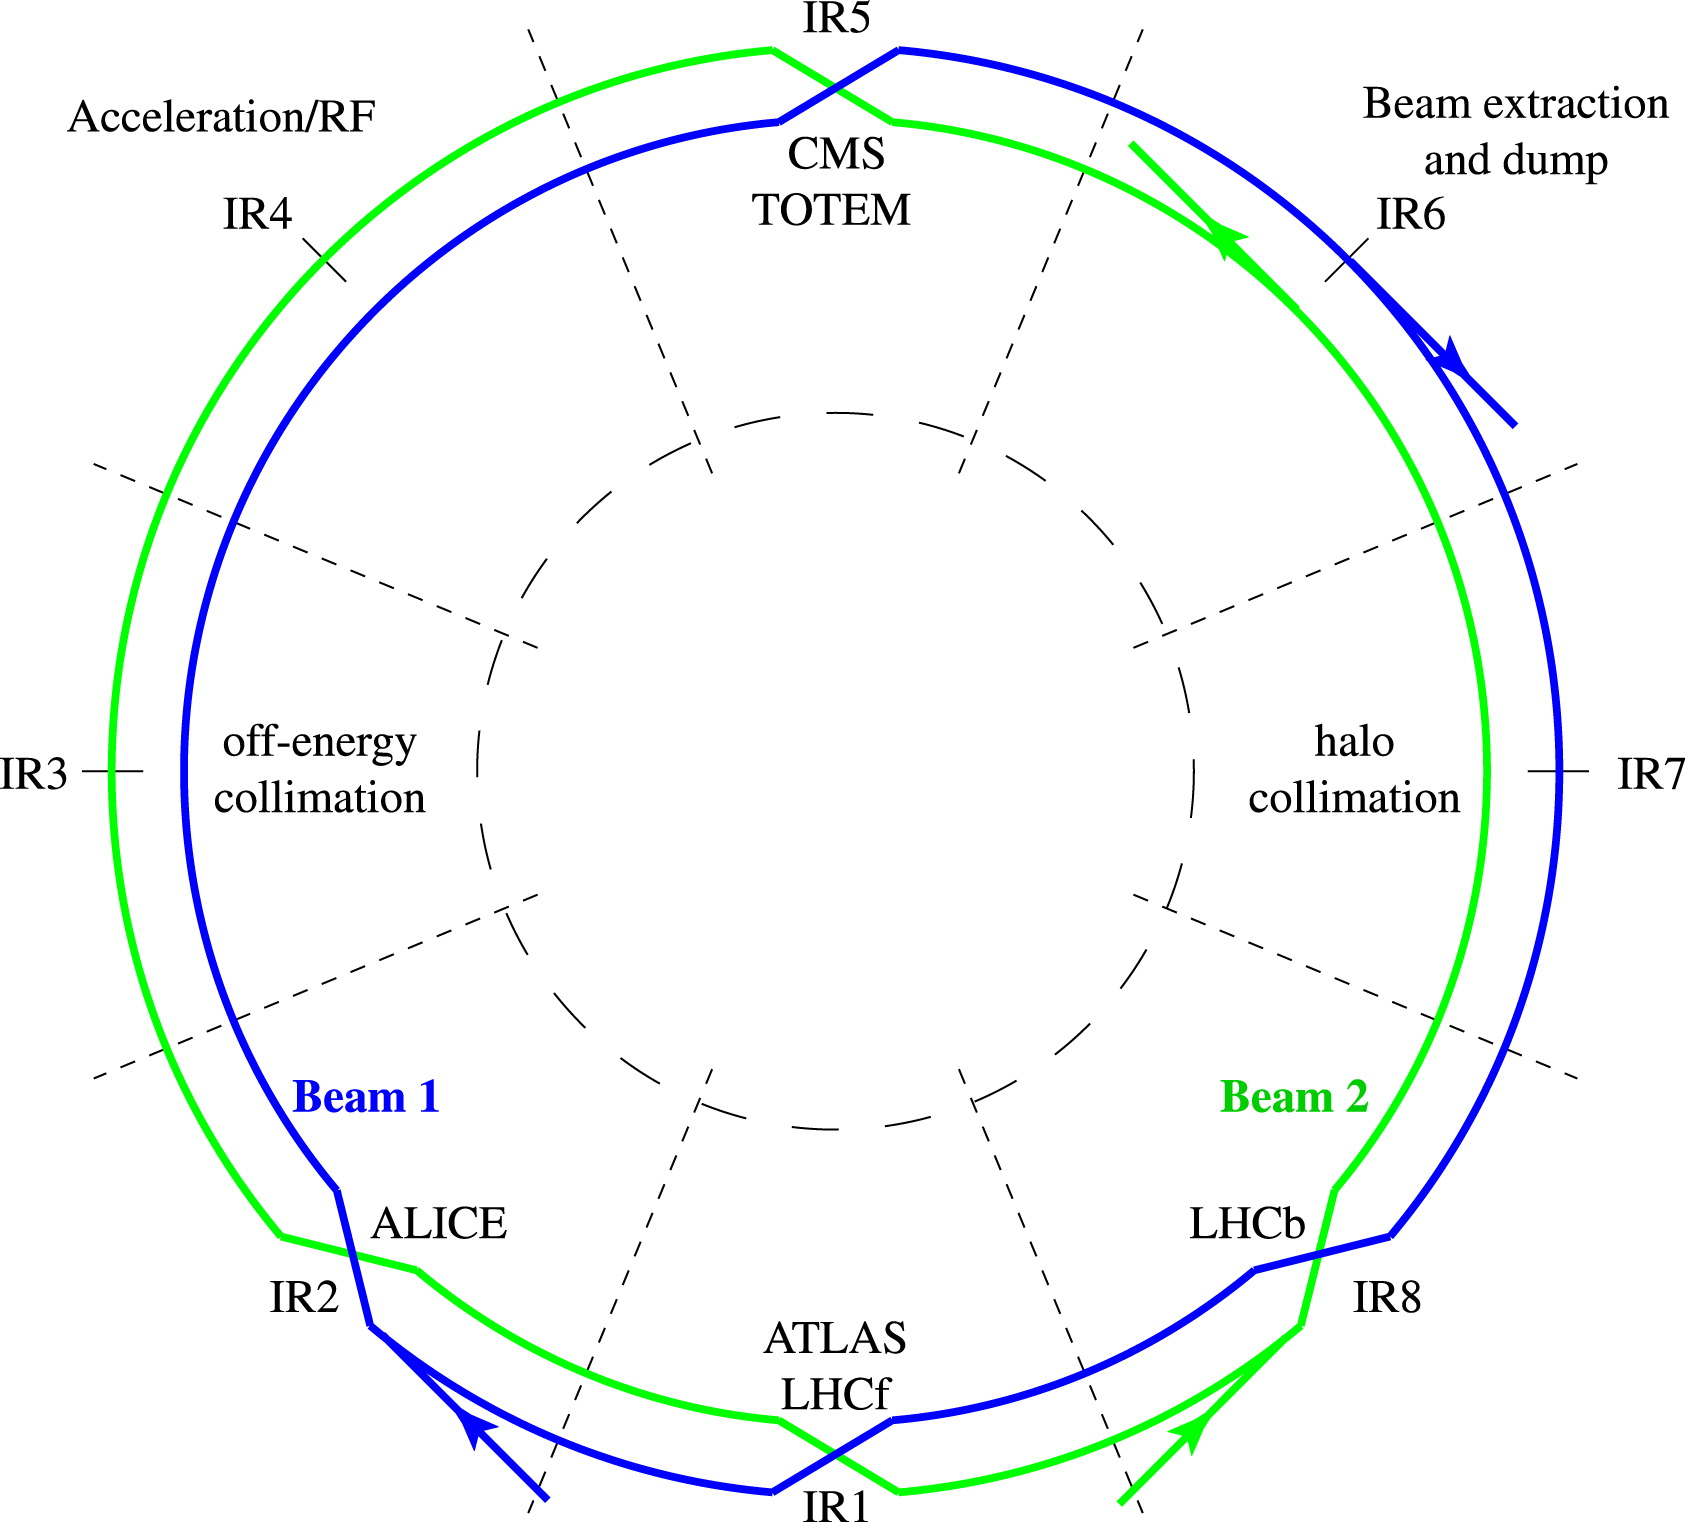
\includegraphics[width= 0.6\textwidth]{Figures/Chapter3/LHC_BasicLayout.jpg}
\caption[Basic schematic layout of the Large Hadron Collider]{Basic schematic layout of the \ac{LHC} consisting of 8 arc sections along with the two circulating beams. The locations of the ATLAS, ALICE, \ac{CMS}, and LHCb experiments are also displayed. Figure taken from Ref.~\cite{LHC_BasicLayout}.}
\label{Figure:Chapter3_LHC_BasicLayout}
\end{figure}

\newpage
Before entering the \ac{LHC} ring, protons are ramped up through a series of pre-accelerator stages. The \ac{LHC} represents the final link in this injector chain~\cite{LHC_InjectorComplex}, as shown in Fig.~\ref{Figure:Chapter3_LHC_Complex}. The first step is the \textbf{\ac{LINAC4}}~\cite{LINAC4}, where hydrogen gas is ionised to produce negative hydrogen ions and accelerated to $160\MeV$ for injection into the \textbf{\ac{PSB}}. During injection into the \ac{PSB}, electrons are stripped off, leaving a pure proton beam that the \ac{PSB} then accelerates to $2.0\GeV$. From there, the beam enters the \textbf{\ac{PS}}, raising its energy to $26\GeV$, before moving on to the \textbf{\ac{SPS}}, which boosts it to $450\GeV$. The beam is then injected into the \ac{LHC}, where its energy is ramped up to several $\TeV$ in less than half an hour.

\begin{figure}[!htbp]
\centering
\includegraphics[width= 0.85\textwidth]{Figures/Chapter3/LHC_AcceleratorComplex.pdf}
\caption[Schematic diagram of the CERN accelerator complex]{Schematic diagram of the \ac{CERN} accelerator complex. Figure taken from Ref.~\cite{LHC_InjectorComplex}.}
\label{Figure:Chapter3_LHC_Complex}
\end{figure}

The \ac{LHC} \textit{functions as a synchrotron accelerator}: protons continuously circulate the ring while radio-frequency (RF) cavities incrementally boost their energy. The strength of the bending magnets increases in synchrony with the rising beam momentum, allowing the particles to remain on a fixed trajectory. A network of 1,232 superconducting niobium-titanium dipole magnets, cooled to $1.9\unit{K}$ with superfluid helium, generates magnetic fields of up to $8.4\unit{T}$ to guide the beams along their circular path. At each of the four principal collision points, inner triplet quadrupole magnets compress the beams to reduce their transverse size, effectively squeezing them to maximise collision rates. These specifications reflect the accelerator complex's capabilities following upgrades completed during the most recent long shutdown.

\subsection{Cross section and Luminosity}

\textit{Cross section} and \textit{luminosity} are essential for predicting collision rates in the detector. The cross-section $\sigma(\sqrt{s})$ describes the probability of a given process occurring at centre-of-mass energy $\sqrt{s}$. However, knowing how often collisions occur also depends on how many particles are available to interact, which is described by the \textit{instantaneous luminosity} ($\mathscr{L}$). This quantity measures the number of particles passing through a unit area per unit time at the interaction point and depends on the detailed structure of the beams.

Since the proton beams at the \ac{LHC} are not continuous streams but are composed of discrete bunches, the temporal structure of the beams directly impacts the collision frequency. Each bunch contains roughly $1.1\times10^{11}$ protons. During Run 2, the beams carried up to 2,040 bunches in 2016 and 2,556 bunches in 2017-2018~\cite{Steerenberg:2696126}. In 2022–2023, this number increased to a maximum of 2,808 bunches per beam, with bunches spaced by $25\unit{ns}$, corresponding to a crossing rate of $40\unit{MHz}$. The number of bunches, the number of protons per bunch, and the bunch spacing together determine the beam intensity and collision frequency, and therefore contribute directly to the luminosity. The dependence of the instantaneous luminosity on the beam parameters can be expressed as:

\begin{equation_pad}
\begin{aligned}
    \mathscr{L} &= \gamma \frac{n_b N^2 f_{\text{rev}}}{4\pi \beta^* \epsilon_n} R \\
    R &= 1 / \sqrt{1 + \left( \frac{\theta_c \sigma_z}{2\sigma} \right) }
\end{aligned}
\end{equation_pad}

where $\gamma$ is the proton beam energy expressed in rest mass units, $n_b$ is the number of bunches per beam, $N$ is the number of particles per bunch, $f_{rev}$ is the revolution frequency, $\beta^*$ is the beam beta function at the collision point and $\epsilon_n$ is the normalised transverse beam emittance. The term R is a geometrical reduction factor for luminosity. This is expressed as a function of the crossing angle of the beams at the collision point ($\theta_c$) and the transverse (longitudinal) spread of the particle bunch, $\sigma_z (\sigma)$. 

Because the beam parameters evolve over time, the luminosity is not constant. Therefore, the more appropriate quantity is the \textit{integrated luminosity} ($\mathscr{L}_{int}$), which represents the total data collected over a given period:

\begin{equation_pad}
    \mathscr{L}_{int} = \int \mathscr{L}(t) dt
\end{equation_pad}

The total number of events $(\mathscr{N})$ for a particular process with cross-section $\sigma$ over a fixed period can then be expressed as:

\begin{equation_pad}
    \mathscr{N} = \sigma \cdot \mathscr{L}_{int}
\end{equation_pad}

A summary of the total integrated luminosity delivered to the \ac{CMS} experiment since 2015 is provided in Fig.~\ref{Figure:Chapter3_CMS_IntegratedLumi}.

\begin{figure}[!htbp]
\centering
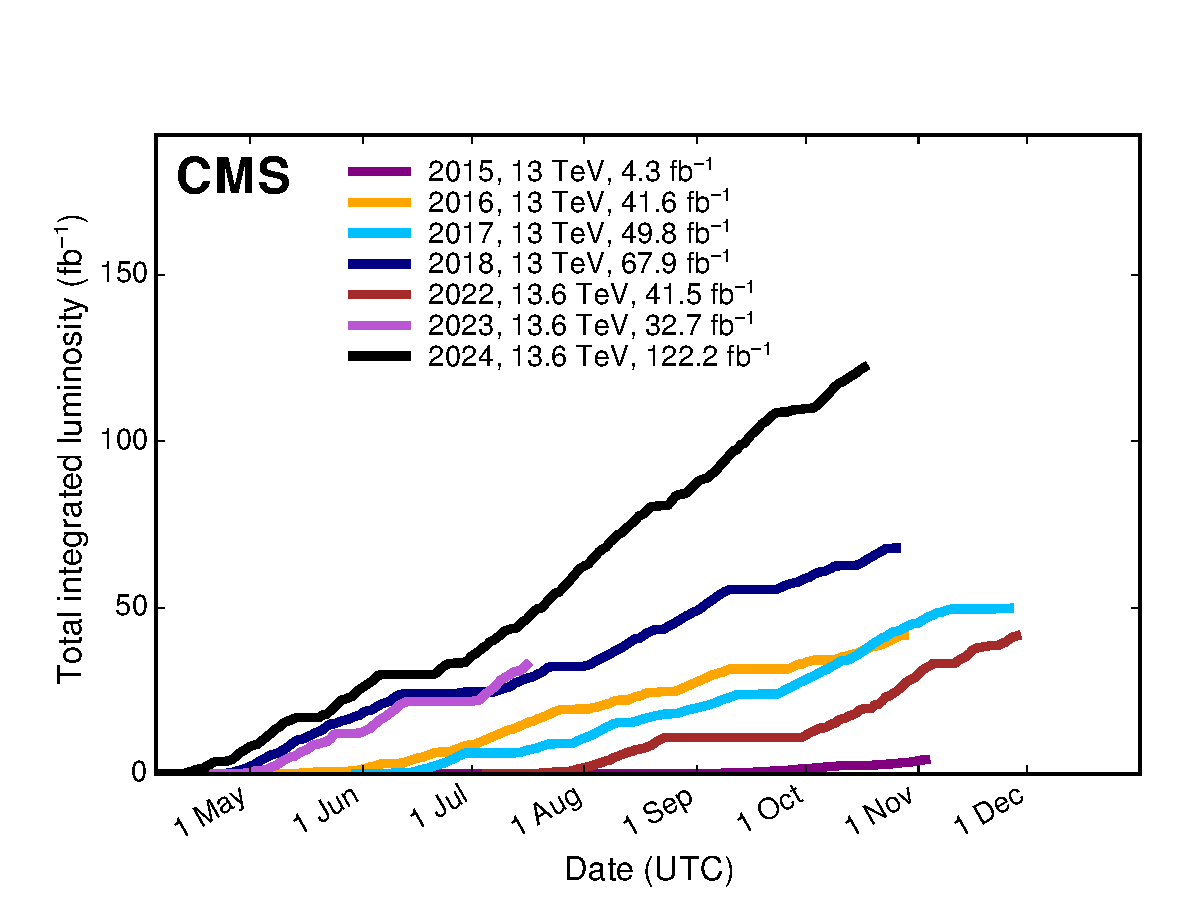
\includegraphics[width= 0.7\textwidth]{Figures/Chapter3/CMS_IntegratedLumi.pdf}
\caption[Total integrated luminosity delivered to the \ac{CMS} experiment between 2015 and 2024]{Total integrated luminosity delivered to the \ac{CMS} experiment between 2015 and 2024. Data collected from all periods except 2015 and 2024 are used in this thesis. Figure taken from Ref.~\cite{CMS_IntegratedLumi}.}
\label{Figure:Chapter3_CMS_IntegratedLumi}
\end{figure}

\subsection{Pileup}

To maximise the probability of observing rare processes, the \ac{LHC} collides large bunches of protons, resulting in high instantaneous luminosity. However, this also introduces challenges: \textit{when bunches collide, multiple protons interact simultaneously, and the vast majority of these pp collisions do not involve a hard scattering process}. This means that for each event, the pp interaction of interest is recorded along with additional pp interactions, called \textbf{\ac{PU}} interactions. 

These \ac{PU} interactions act as background noise, complicating the reconstruction of the primary hard-scattering event and degrading the performance of many physics measurements. As instantaneous luminosity increases, \ac{PU} becomes more severe, and removing the unwanted overlap collisions requires increasingly sophisticated mitigation techniques. Figure~\ref{Figure:Chapter3_CMS_Pileup} displays the \ac{PU} conditions encountered by the \ac{CMS} experiment between 2015 and 2024.

\begin{figure}[!htbp]
\centering
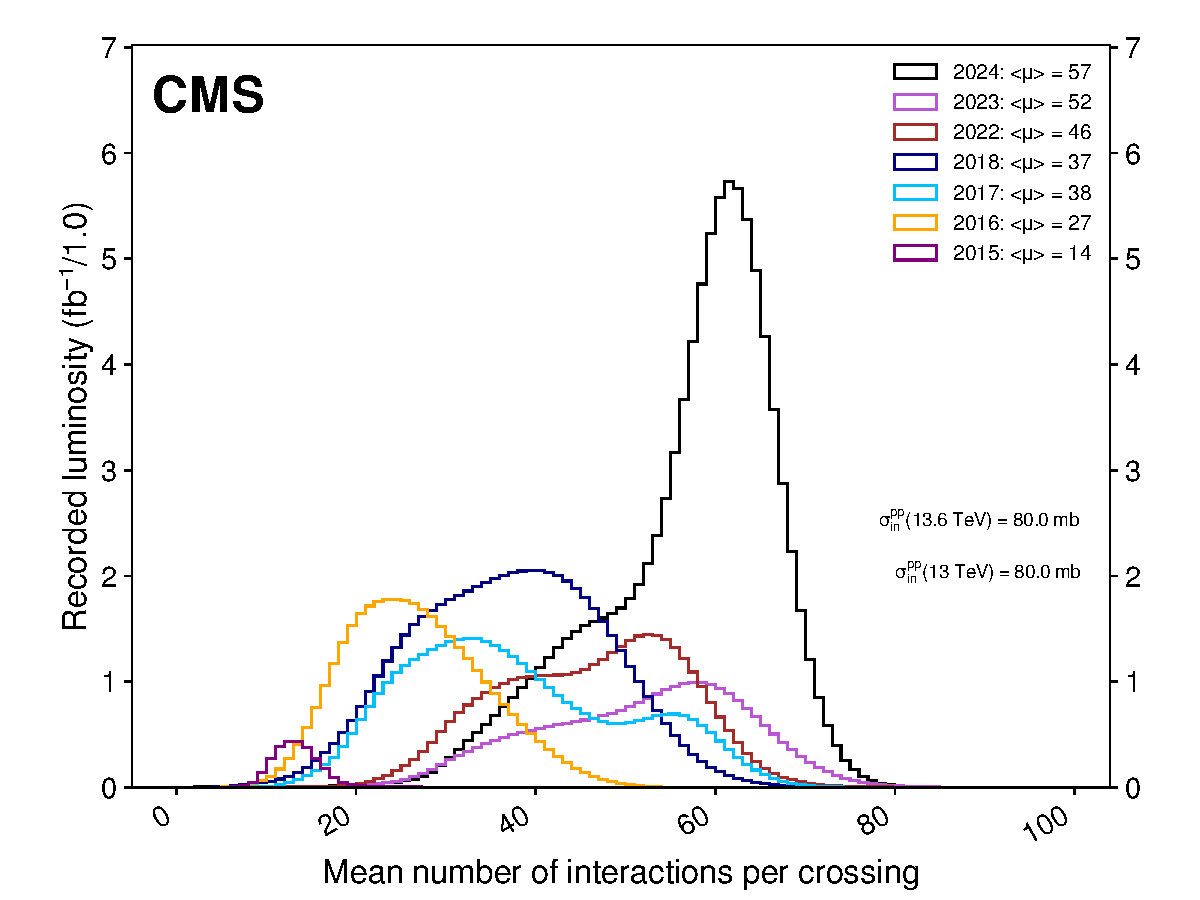
\includegraphics[width= 0.7\textwidth]{Figures/Chapter3/CMS_Pileup.pdf}
\caption[Distribution of the average number of interactions per bunch crossing for pp collisions at CMS between 2015 and 2024]{Distribution of the average number of interactions per bunch crossing for pp collisions between 2015 and 2024, using data from the \ac{CMS} experiment. Figure taken from Ref.~\cite{CMS_IntegratedLumi}.}
\label{Figure:Chapter3_CMS_Pileup}
\end{figure}

\section{The CMS Detector}
\label{Section:Chapter3_CMS_Detector_Introduction}
\ac{CMS} is one of the two general-purpose detectors at the \ac{LHC}, built to explore a wide range of high-energy physics phenomena. The design of the \ac{CMS} detector was shaped by the ambitious goals of the \ac{LHC} physics programme~\cite{LHC_CMS}, which demanded precise and efficient measurements under challenging experimental conditions. To accomplish these objectives, several key performance requirements were identified:

\begin{itemize}
  \item Identification \& precise momentum reconstruction of muons over a broad range of momenta and angles; dimuon mass resolution $\sim1\%$ at $100\GeV$; unambiguous muon charge identification up to $1\TeV$
  \item High momentum resolution \& reconstruction efficiency for charged particles; efficient $\tau$-lepton and b‐jet identification
  \item Photon/electron energy measurement with excellent resolution; diphoton and dimuon mass resolution $\sim1\%$ at $100\GeV$ over a wide geometrical coverage
  \item Effective $\pi^0$ rejection; efficient isolation of photons and leptons in high‐luminosity, high‐occupancy conditions
  \item Precise dijet mass reconstruction and good \ac{MET} resolution
\end{itemize}

\ac{CMS} employs a compact, layered detector system arranged cylindrically around the interaction point to fulfil these performance requirements, providing nearly 4$\pi$ solid-angle coverage. The entire detector is $21.6\unit{m}$ long and has a diameter of $14.6\unit{m}$ while weighing $12,500\unit{t}$. This makes \ac{CMS} one of the largest yet compact detectors ever engineered for a particle physics experiment. Closest to the beam pipe lies the \textbf{silicon tracker}, which precisely tracks charged particles. It is surrounded by the \textbf{\ac{ECAL}}, optimised for measuring the energy of electrons and photons with high precision. The \textbf{\ac{HCAL}} follows and is responsible for absorbing and measuring the energy of hadrons. These three subdetectors are enclosed within a powerful $13\unit{m}$ long, $6\unit{m}$ inner-diameter, $3.8\unit{T}$ \textbf{superconducting solenoid}. Embedded within the iron return yoke of the solenoid is the \textbf{muon detection system}. A schematic of the full \ac{CMS} detector is shown in Fig.~\ref{Figure:Chapter3_CMS_schematic}, providing an overview of its cylindrical geometry and layered structure around the \ac{LHC} interaction point. The following sections will provide a more detailed discussion of each of the major subdetector systems introduced here. A complementary longitudinal slice through the detector is shown in Fig.~\ref{Figure:Chapter3_CMS_slice}, serving as a visual reference for the detailed subdetector descriptions that follow.

\begin{figure}[!htbp]
\centering
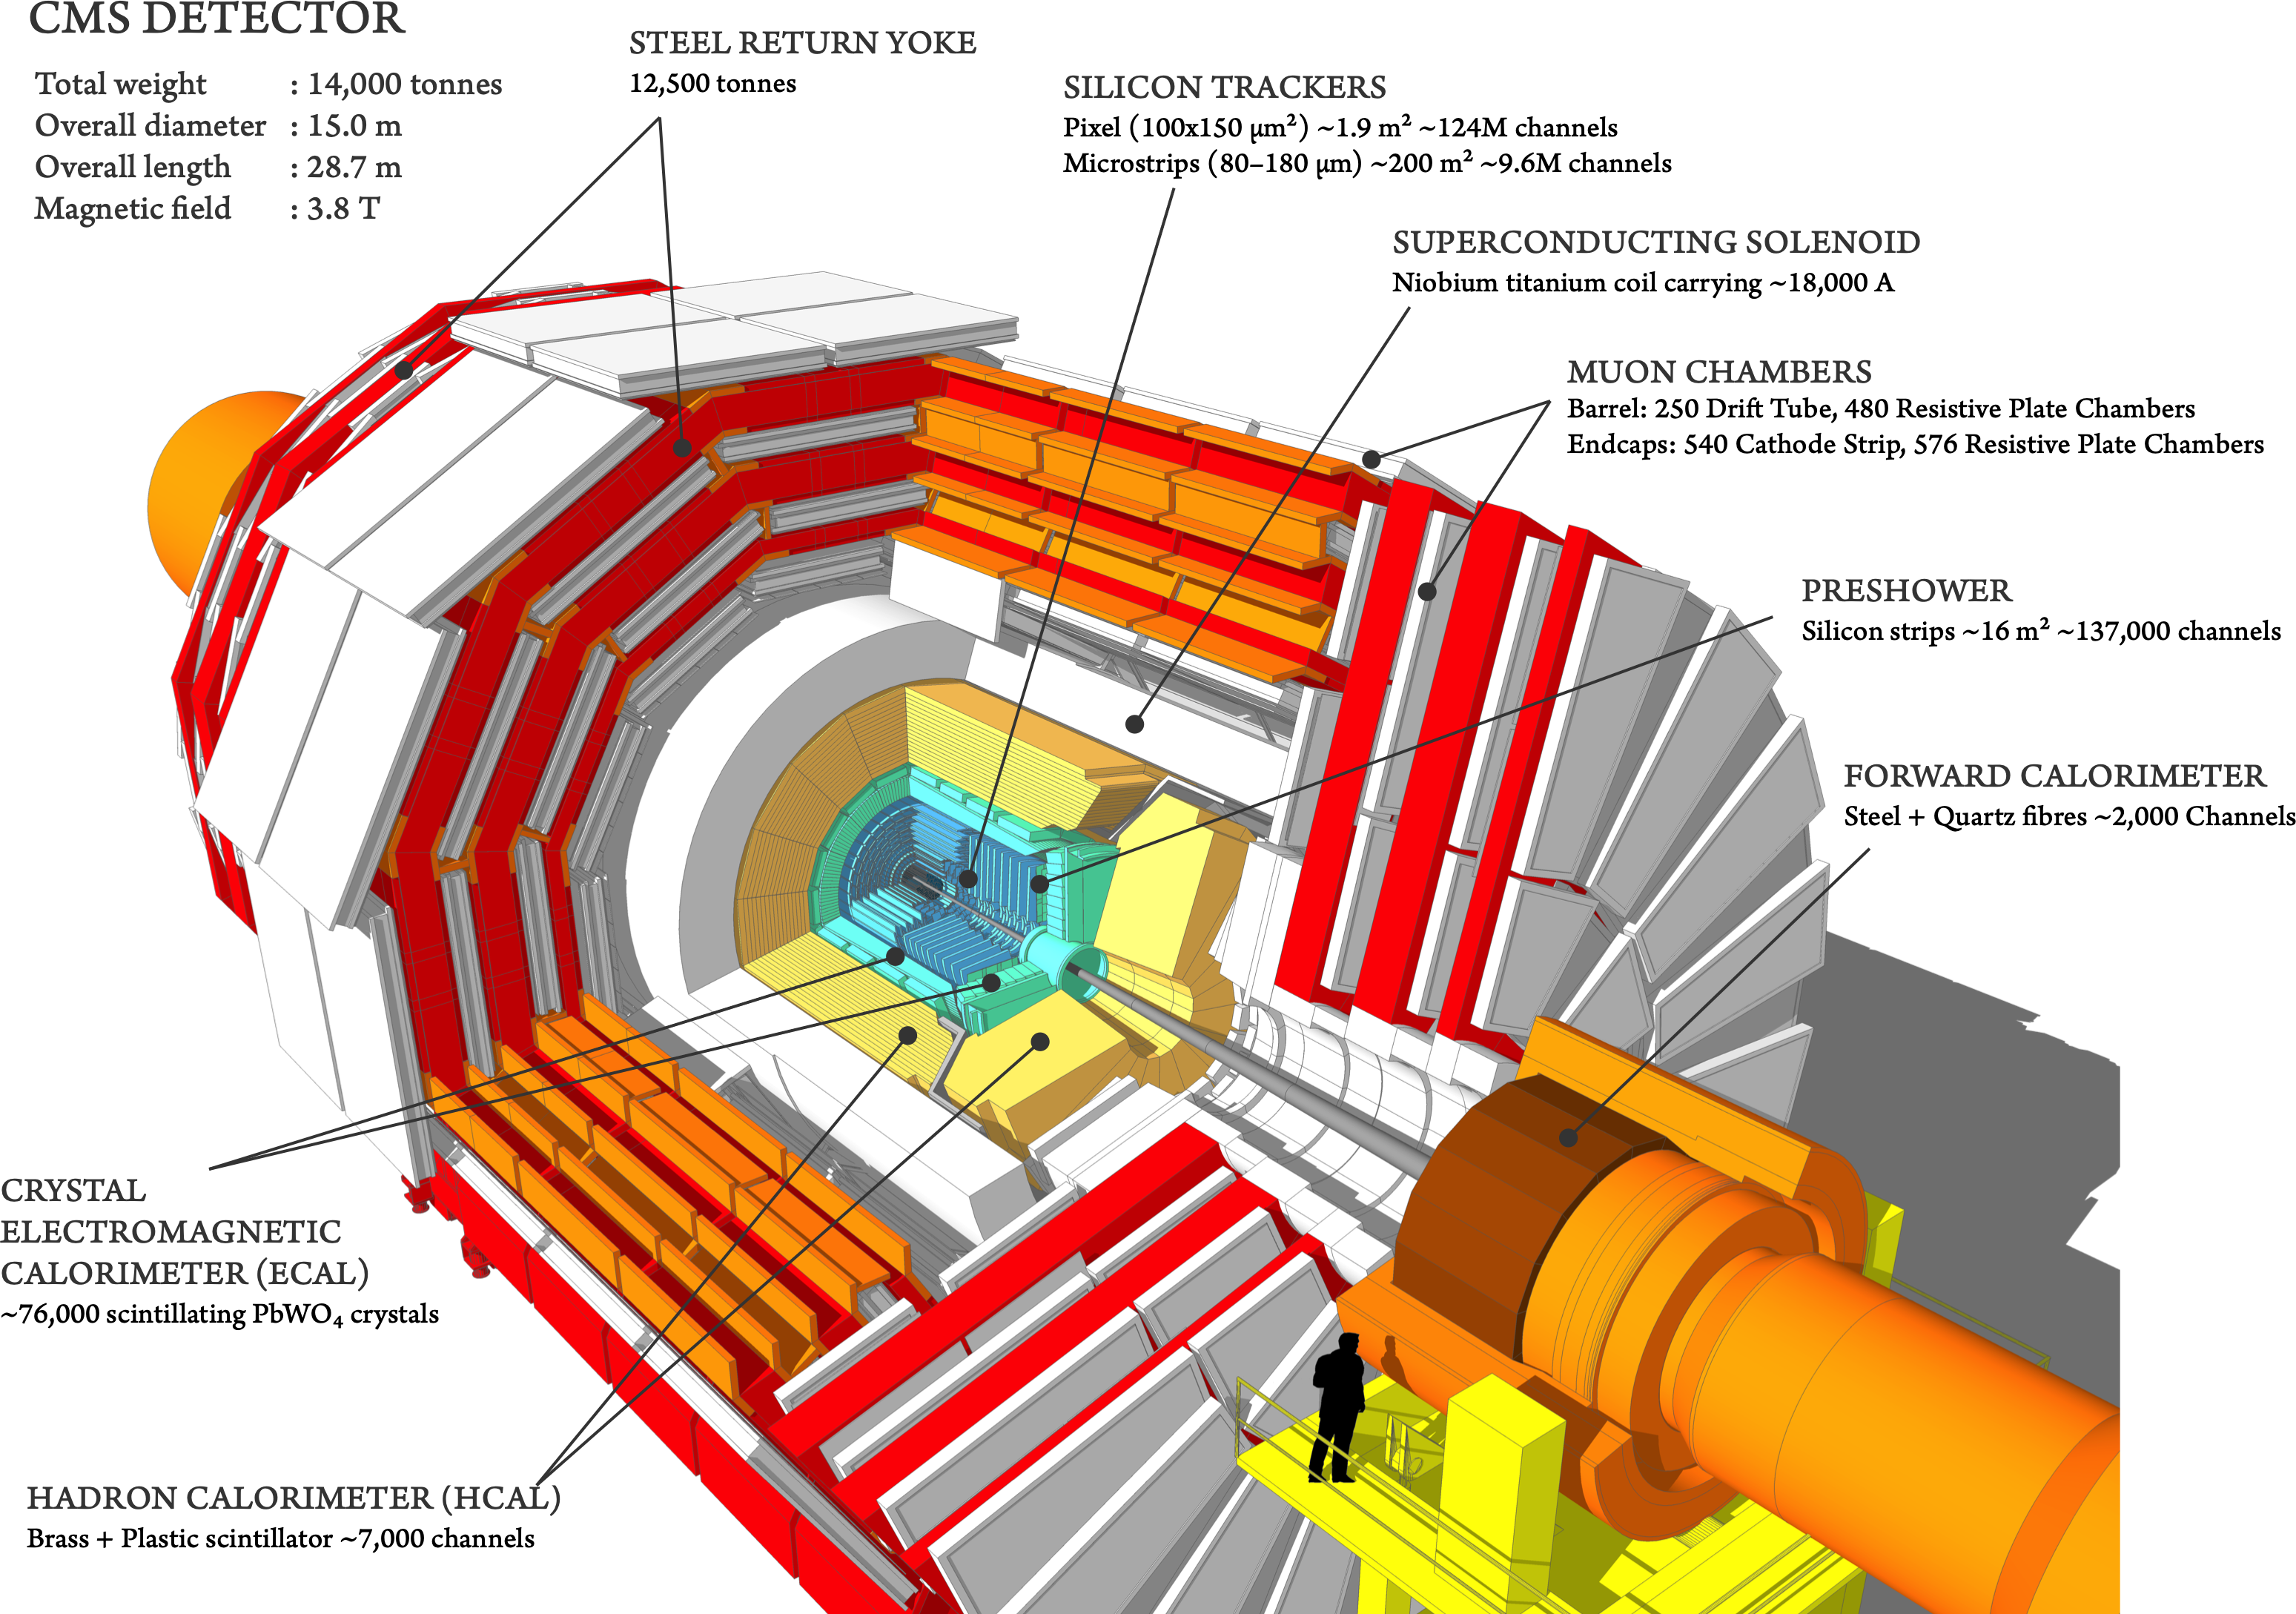
\includegraphics[width= 0.8\textwidth]{Figures/Chapter3/CMS_Detector.pdf}
\caption[Schematic drawing of the CMS detector]{Schematic drawing of the \ac{CMS} detector. Figure taken from Ref.~\cite{CMS_Detector_Run3}.}
\label{Figure:Chapter3_CMS_schematic}
\end{figure}

\begin{figure}[!htbp]
\centering
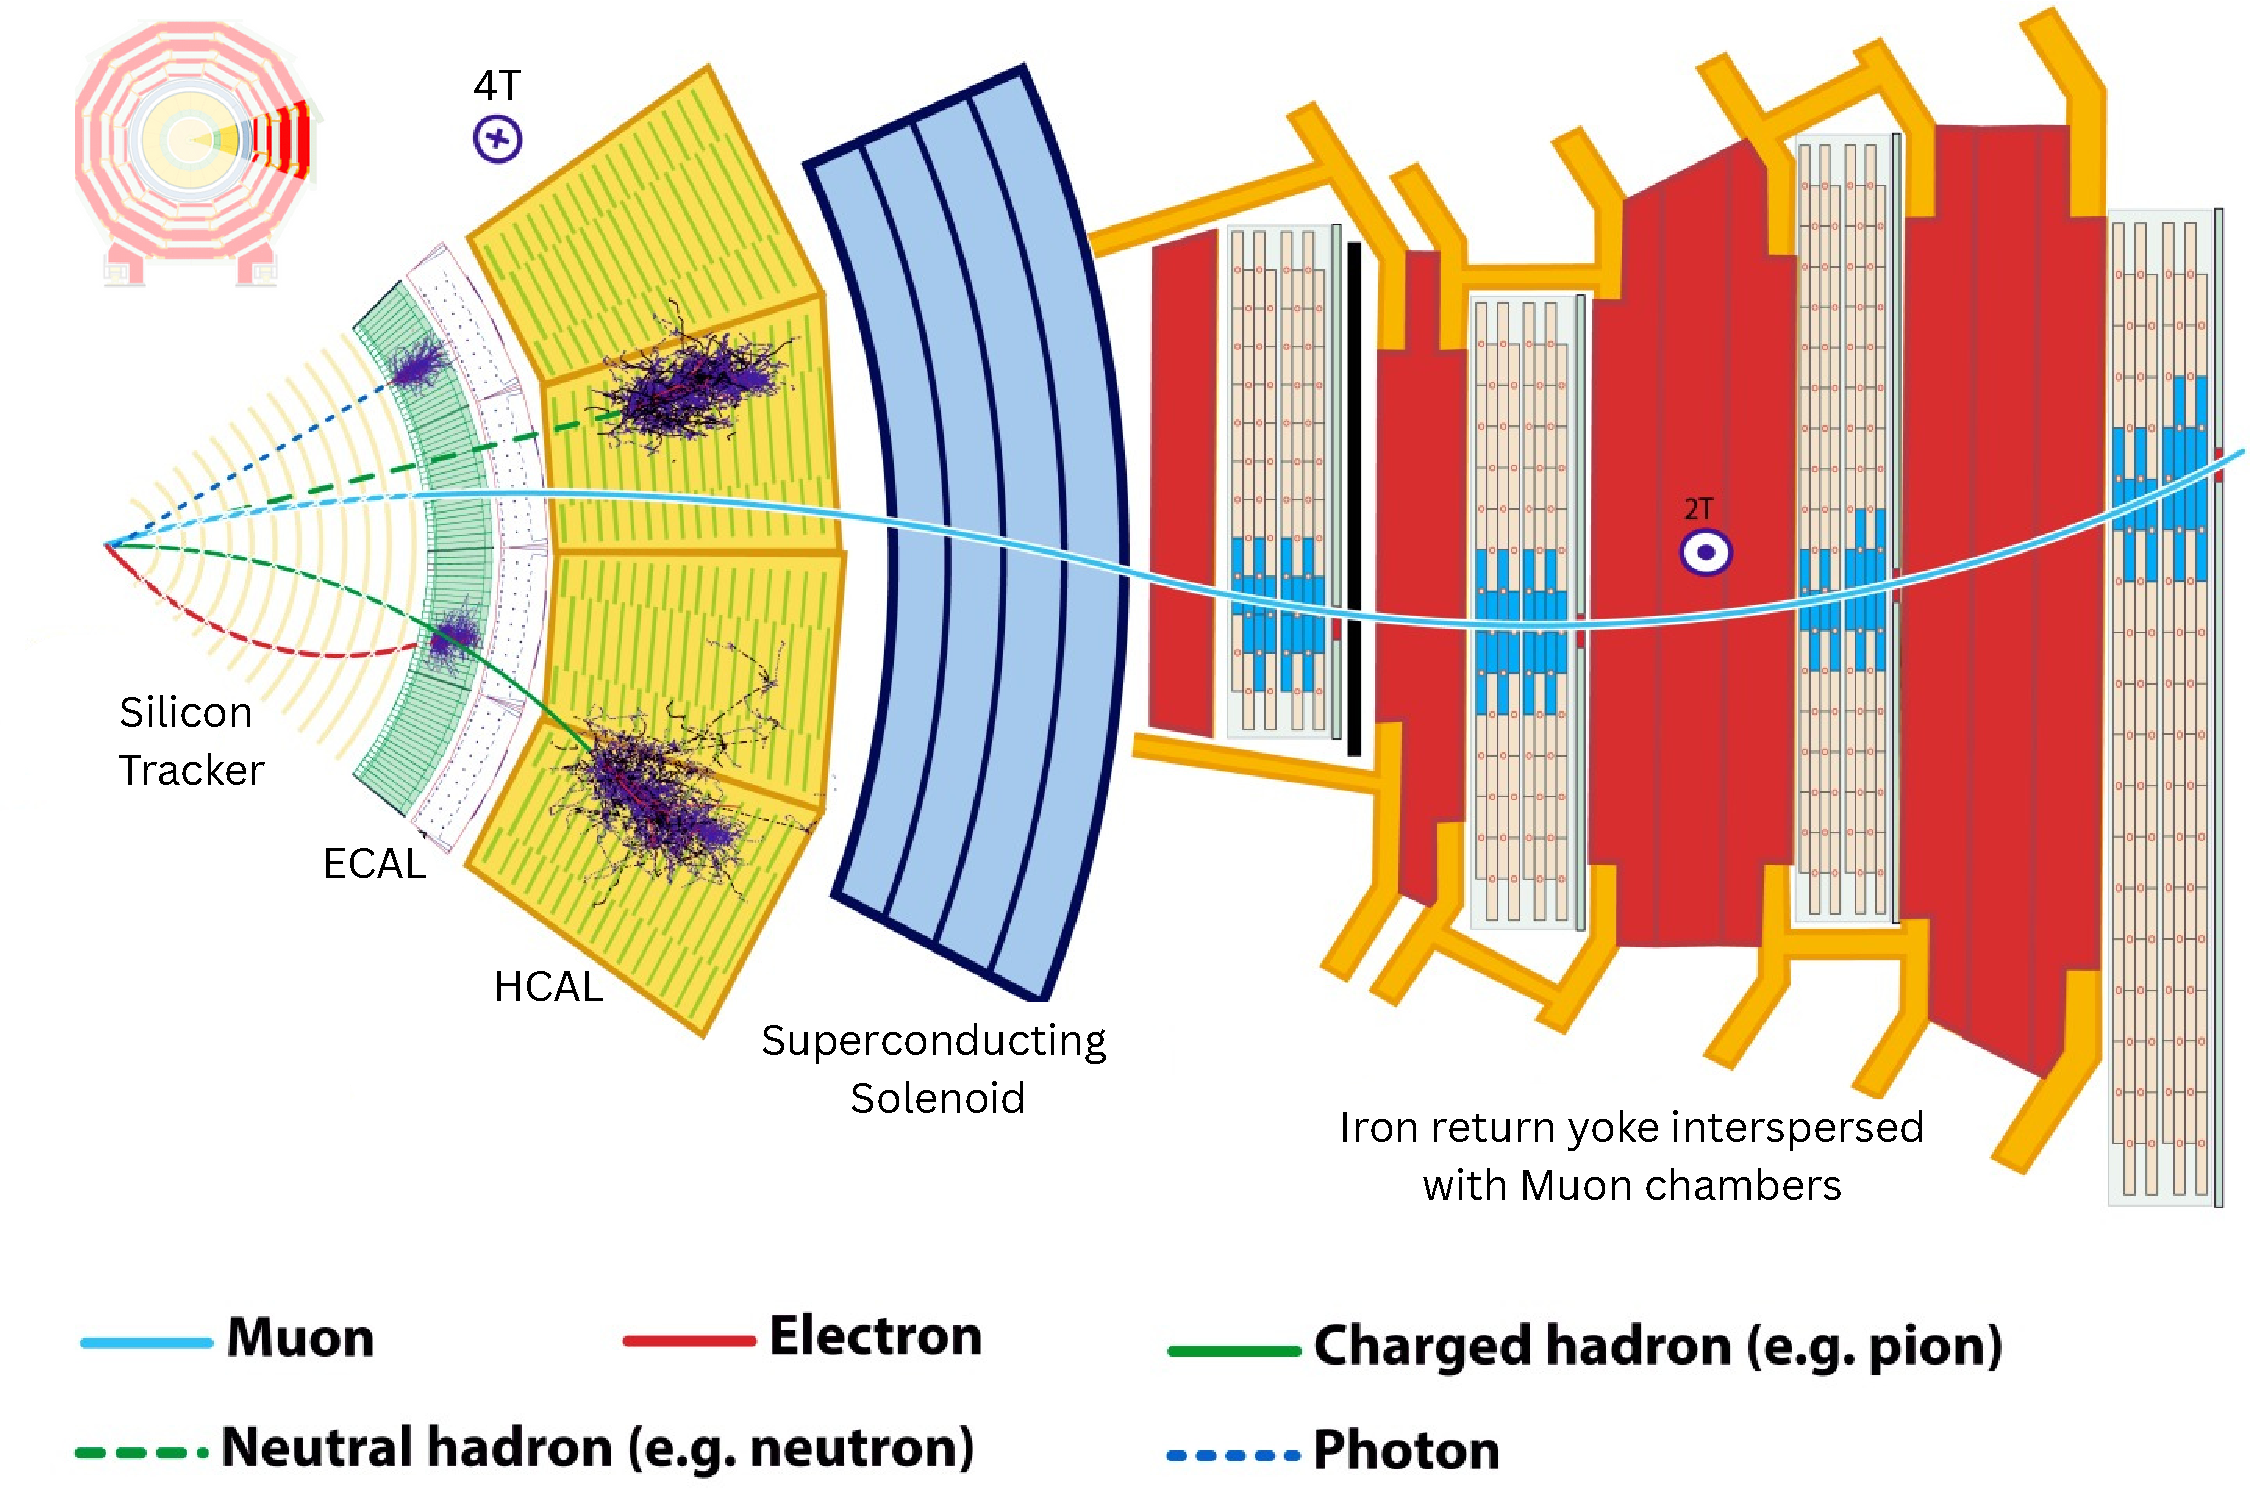
\includegraphics[width= 0.8\textwidth]{Figures/Chapter3/CMS_Detector_Slice.pdf}
\caption[Transverse slice of the CMS detector]{A transverse slice of the \ac{CMS} detector displaying the individual subsystems and their response to different types of particles. Figure adjusted from Ref.~\cite{CMS_Detector_Slice}.}
\label{Figure:Chapter3_CMS_slice}
\end{figure}

\clearpage
\subsection{Co-ordinate system}
\ac{CMS} adopts a right-handed Cartesian coordinate system centred at the nominal collision point. The $x$-axis points towards the centre of the \ac{LHC} ring, and the $y$-axis points vertically upwards, while the $z$-axis points along the beam direction towards the Jura mountains, as illustrated in Fig.~\ref{Figure:Chapter3_CMS_CoordinateSystem}.

\begin{figure}[!htbp]
\centering
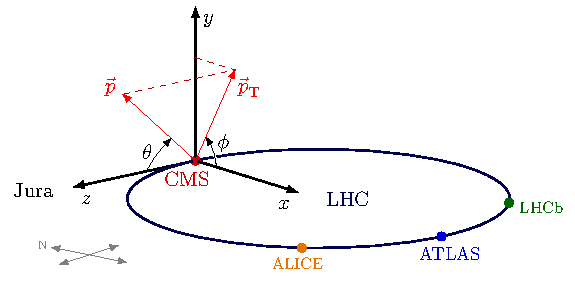
\includegraphics[width= 0.8\textwidth]{Figures/Chapter3/CMS_CoordinateSystem.pdf}
\caption{The CMS detector coordinate system.}
\label{Figure:Chapter3_CMS_CoordinateSystem}
\end{figure}

In this system, the plane perpendicular to the beam axis, $x$-$y$ plane, is referred to as the \textit{transverse plane}, while the $z$-axis defines the \textit{longitudinal direction}. The \textit{azimuthal angle} $\phi \in [0,2\pi]$ is the angle with respect to the positive $x$-axis in the transverse plane, while the \textit{polar angle} $\theta \in [0,\pi]$ is with respect to the $z$-axis. Rather than using $\theta$ directly, it is common in collider physics to introduce \textit{pseudorapidity} ($\eta$), defined as

\begin{equation_pad}
    \eta = - \ln\left[\tan(\theta/2)\right]
\end{equation_pad}

A key property of this quantity is that the difference in pseudorapidity ($\Delta\eta$) between two vectors is invariant under Lorentz boosts along the longitudinal $z$-axis. This is convenient in hadron collider experiments, where the parton-parton centre-of-mass frame is often significantly boosted along the beam direction due to the variable momentum fractions carried by the incoming partons. Additionally, $\eta$ provides a nearly linear mapping of $\theta$ (shown in Fig.~\ref{Figure:Chapter3_Pseudorapidity}), facilitating a simple description of particle emission angles relative to the beam axis. This property allows for a natural segmentation of the detector into barrel and endcap regions based on $\eta$.

\begin{itemize} 
\item \textbf{Barrel region}: The central cylindrical region of the detector, located closest to the primary interaction point and optimised for particles emitted at large angles to the beamline ($\ie$ low $|\eta|$). 
\item \textbf{Endcap regions}: Located at either end of the barrel along the $z$-axis, designed to detect particles emitted at small angles with respect to the beamline ($\ie$ high $|\eta|$). 
\end{itemize}

\begin{figure}[!htbp]
\centering
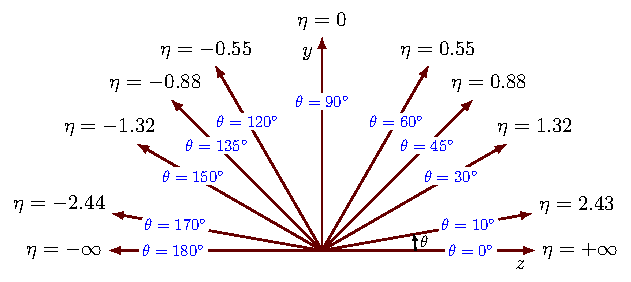
\includegraphics[width= 0.8\textwidth]{Figures/Chapter3/Pseudorapidity.pdf}
\caption{Illustration of the relationship between pseudorapidity ($\eta$) and polar angle ($\theta$).}
\label{Figure:Chapter3_Pseudorapidity}
\end{figure}

At the \ac{LHC}, the initial momentum component of the system perpendicular to the beam axis is nearly zero because of the head-on nature of the beam. This kinematic quantity is referred to as the transverse momentum ($p_\mathrm{T}$) and is defined as:

\begin{equation_pad}
    p_\mathrm{T} = \sqrt{p_x^2 + p_y^2}
\end{equation_pad}

Transverse momentum is a central observable in collider physics. It provides a direct probe of hard interaction processes characterised by large momentum transfers. A complementary quantity to the transverse momentum is the missing transverse momentum ($E_\mathrm{T}^{\text{miss}}$), which is defined as the negative vector sum of the transverse momenta of all reconstructed particles in an event. This is a critical quantity serving as an estimator of the transverse momentum carried by non-interacting or undetected particles.

The radial distance from the beam axis is typically expressed as $r = \sqrt{x^2+y^2}$. Additionally, it is also convenient to express the distance metric ($\Delta R$) between two objects in a Lorentz-invariant way as:

\begin{equation_pad}
    \Delta R = \sqrt{(\Delta\eta)^2 + (\Delta \phi)^2}
\end{equation_pad}

This quantity is important in object reconstruction, as discussed in Chapter~\ref{Section:Chapter4}.%

\subsection{Magnet System}

As its name implies, \ac{CMS} is defined by its central feature: the solenoid magnet. This critical component generates a very strong magnetic field that bends the trajectories of charged particles as they traverse the detector. This enables precise measurements of their momenta and electric charges. 

The \textbf{solenoid} spans $13\unit{m}$ in length and $6\unit{m}$ in diameter, capable of producing a magnetic field of up to $4\unit{T}$, but is currently operated at $3.8\unit{T}$ for enhanced long-term stability. The strong field ensures that low-momentum charged particles are sufficiently curved, confining them within the inner tracking system and aiding in precise momentum resolution. This not only improves tracking quality but also helps mitigate calorimeter noise by preventing soft particles from reaching the calorimeters.

Outside the solenoid, the muon detection system is embedded within segmented layers of iron, forming the \textbf{iron yoke}. This massive structure, weighing approximately $10,000\unit{t}$, serves two primary purposes: it returns about two-thirds of the magnetic flux generated inside the detector and provides structural support for the muon chambers. By returning the flux, the iron yoke significantly reduces the magnetic field outside the detector. This magnetic field configuration causes a ``\textit{double bending}'' of muon trajectories: first in one direction as muons pass through the inner silicon tracker, and then in the opposite direction as they traverse the muon chambers embedded in the iron yoke. This double bending significantly enhances the overall muon momentum resolution.
 
\subsection{Inner tracking system}
The \ac{CMS} interaction point is surrounded by the innermost subdetector, the \textbf{silicon tracker}, which measures $5.8\unit{m}$ in length and $2.5\unit{m}$ in diameter~\cite{LHC_CMS,CMS_Detector_Run3}. The tracker plays a central role in reconstructing the trajectories of charged particles and in identifying both primary and secondary interaction vertices with high spatial precision.

At the \ac{LHC}’s design luminosity, on the order of $10^3$ charged particles traverse the tracker volume per each $25\unit{ns}$ bunch crossing. To cope with the extreme occupancy, the tracker must combine high granularity with rapid signal readout. Furthermore, its proximity to the interaction point exposes it to a harsh radiation environment, necessitating the use of radiation-hard sensor technologies to preserve long-term performance.

To meet these demanding requirements, the \ac{CMS} tracker employs \textit{silicon-based sensors}. However, these silicon sensors also require dedicated readout electronics and active cooling systems. These components contribute to the non-active material within the tracking volume, which must be carefully controlled. Excessive material leads to increased multiple scattering and energy loss, degrading momentum resolution and negatively impacting the performance of outer subdetectors such as the calorimeters.

As shown in Fig.~\ref{Figure:Chapter3_Tracker_MaterialBudget}, the material budget of the tracker is kept as low as possible, particularly in the central (low-$\eta$) region of the pixel detector, where precision tracking is most critical.

\begin{figure}[!htbp]
    \centering
    % First row
    \begin{subfigure}[b]{0.49\textwidth}
        \centering
        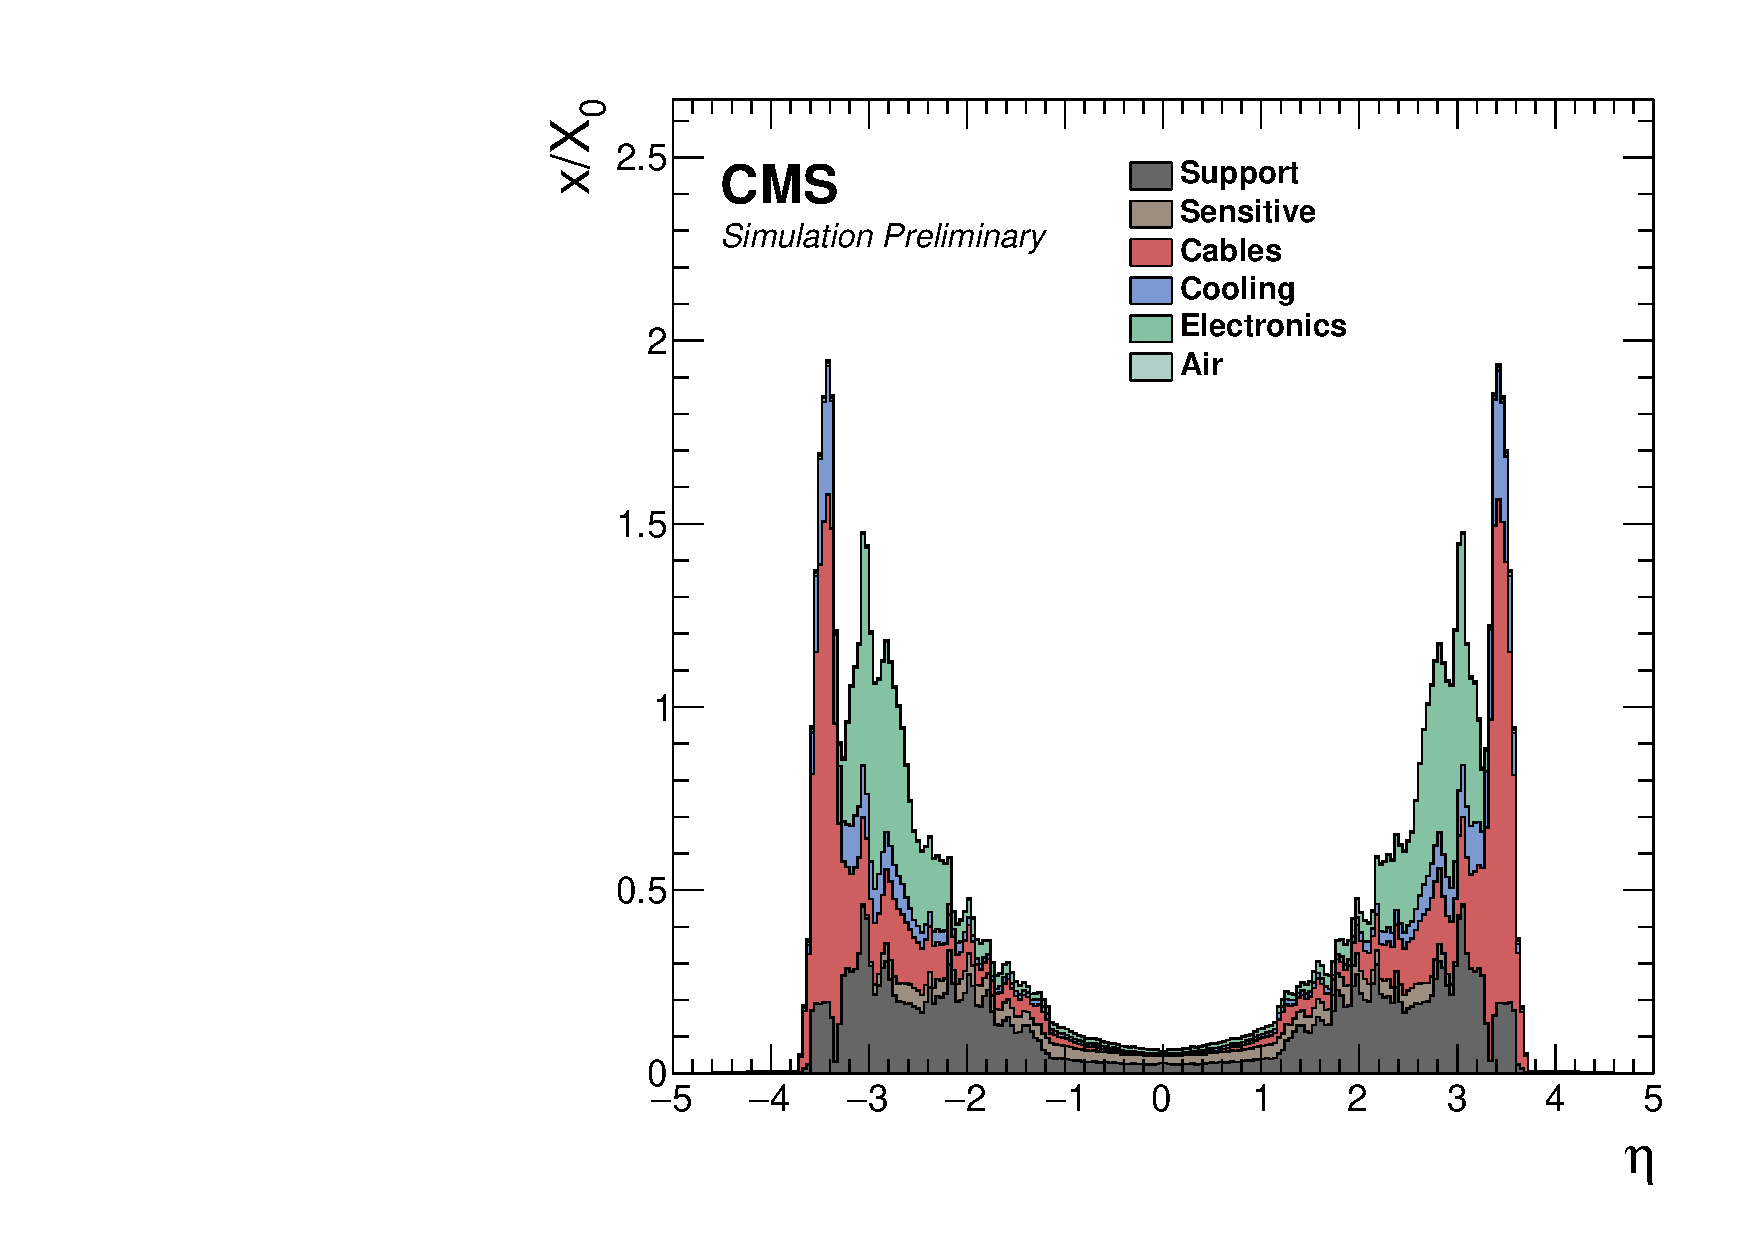
\includegraphics[width=\textwidth]{Figures/Chapter3/Material_Budget1.pdf}
        \caption{}
    \end{subfigure}
    \begin{subfigure}[b]{0.49\textwidth}
        \centering
        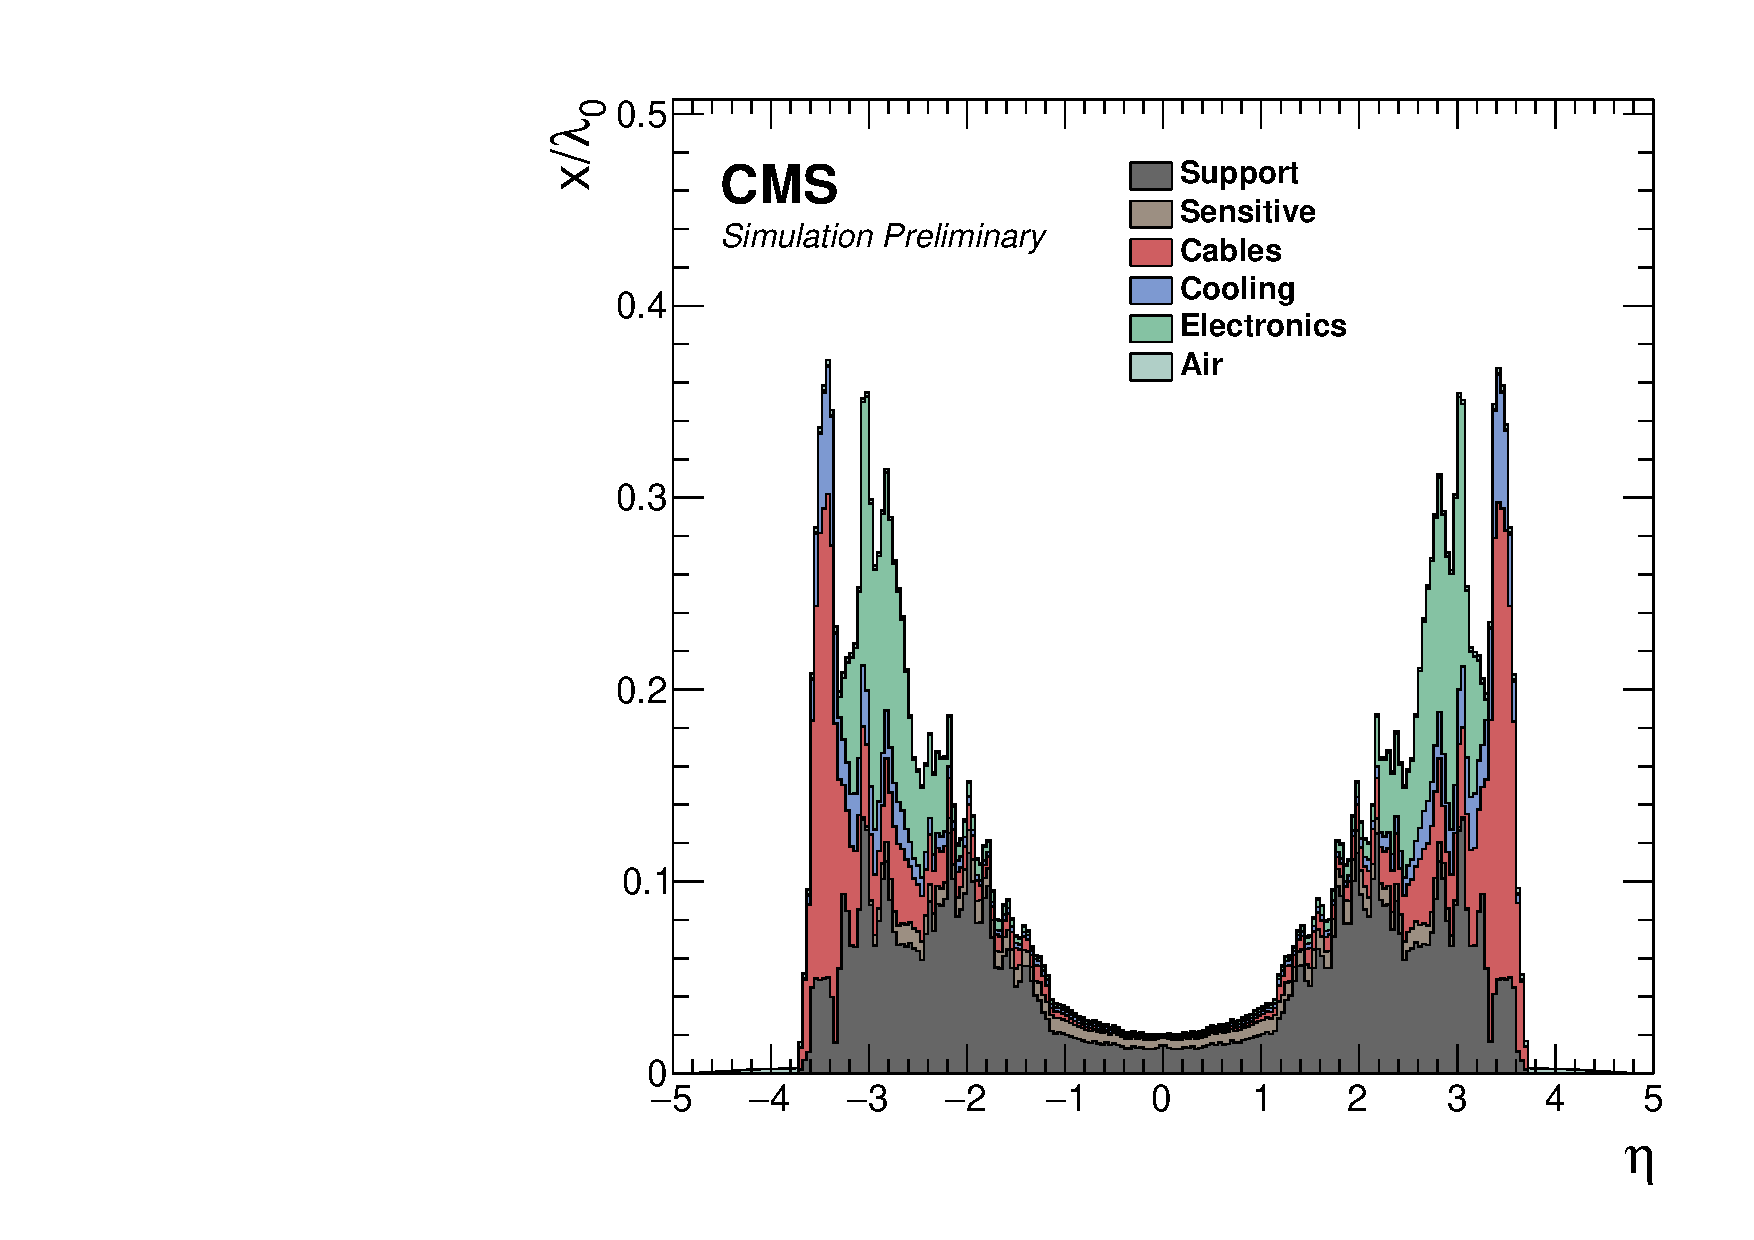
\includegraphics[width=\textwidth]{Figures/Chapter3/Material_Budget2.pdf}
        \caption{}
    \end{subfigure}
\caption[Simulation of the CMS pixel detector material budget]{Simulation of the \ac{CMS} pixel detector material budget as a function of $\eta$ in units of ($\textbf{a}$) radiation length and ($\textbf{b}$) hadronic interaction length for different detector components. Figure taken from Ref.~\cite{TrackerMaterialBudget_Pixel}.}
\label{Figure:Chapter3_Tracker_MaterialBudget}
\end{figure}

\newpage
\subsubsection{Pixel Detector}

The innermost component of the \ac{CMS} tracking system is the \textbf{silicon pixel detector}. The original pixel detector~\cite{LHC_CMS}, installed in 2008, was designed to operate for up to ten years under the \ac{LHC}’s nominal instantaneous luminosity of $1 \times 10^{34}\unit{cm}^{-2}\unit{s}^{-1}$, with the capacity to handle up to 25 \ac{PU} interactions per bunch crossing. However, even during Run-1, the \ac{LHC} exceeded its design luminosity, exposing the pixel detector to increased radiation levels and causing rising readout inefficiencies. To maintain high tracking efficiency under upgraded luminosity conditions of up to $2 \times 10^{34}~\unit{cm}^{-2}\unit{s}^{-1}$ and \ac{PU} levels of 50 or more, the \ac{CMS} pixel detector underwent a major upgrade in 2017, referred to as the Phase-1 upgrade~\cite{CMS_Detector_Run3, CMS_Tracker_Phase1_Upgrade,CMS_Tracker_Phase1_Upgrade_2}. This upgrade introduced a more granular and radiation-tolerant detector layout, featuring four barrel layers and three endcap disks.

The \textbf{\ac{BPIX}} detector consists of four concentric cylindrical layers (L1-L4) positioned at radii of 29, 68, 109, and 160$\unit{mm}$ from the beamline. A total of 1,184 sensor modules are deployed in the barrel region. Each module contains a silicon sensor segmented into $160 \times 416$ individual pixels with a pitch of $100 \times 150\unit{\mu m}^2$, enabling high-resolution hit detection. Compared to the original pixel detector, the innermost layer (L1) was also moved closer to the interaction point by reducing the \ac{CMS} beam pipe radius from 30 to 23$\unit{mm}$ in 2014. 

The \textbf{\ac{FPIX}} detector complements the barrel coverage by extending tracking capabilities in the forward region. It comprises three endcap disks on each side of the detector, located at distances of 291, 396, and 516$\unit{mm}$ from the interaction point. The forward region is equipped with 672 pixel modules, featuring the same fine segmentation and pixel pitch as the barrel modules. Together, the \ac{BPIX} and \ac{FPIX} systems provide approximately 124 million readout channels, ensuring precise tracking throughout the detector’s angular coverage.

The Phase-1 upgrade of the \ac{CMS} pixel detector introduced significant improvements in geometry and coverage, as illustrated in Fig.~\ref{Figure:Chapter3_Pixel_Upgrade}. Additionally, substantial gains were also achieved in spatial resolution and tracking performance. The position resolution reaches approximately $11\unit{\mu m}$ in the $r$-$\phi$ direction and $24\unit{\mu m}$ in the $z$ direction for \ac{BPIX} L3~\cite{CMS_Detector_Run3}. Somewhat worse resolutions are observed in the innermost barrel layers due to higher radiation damage. For \ac{FPIX}, the corresponding resolutions are about $12\unit{\mu m}$ ($r$) and $21\unit{\mu m}$ ($z$)~\cite{CMS_Detector_Run3}. 

\begin{figure}[!htbp]
\centering
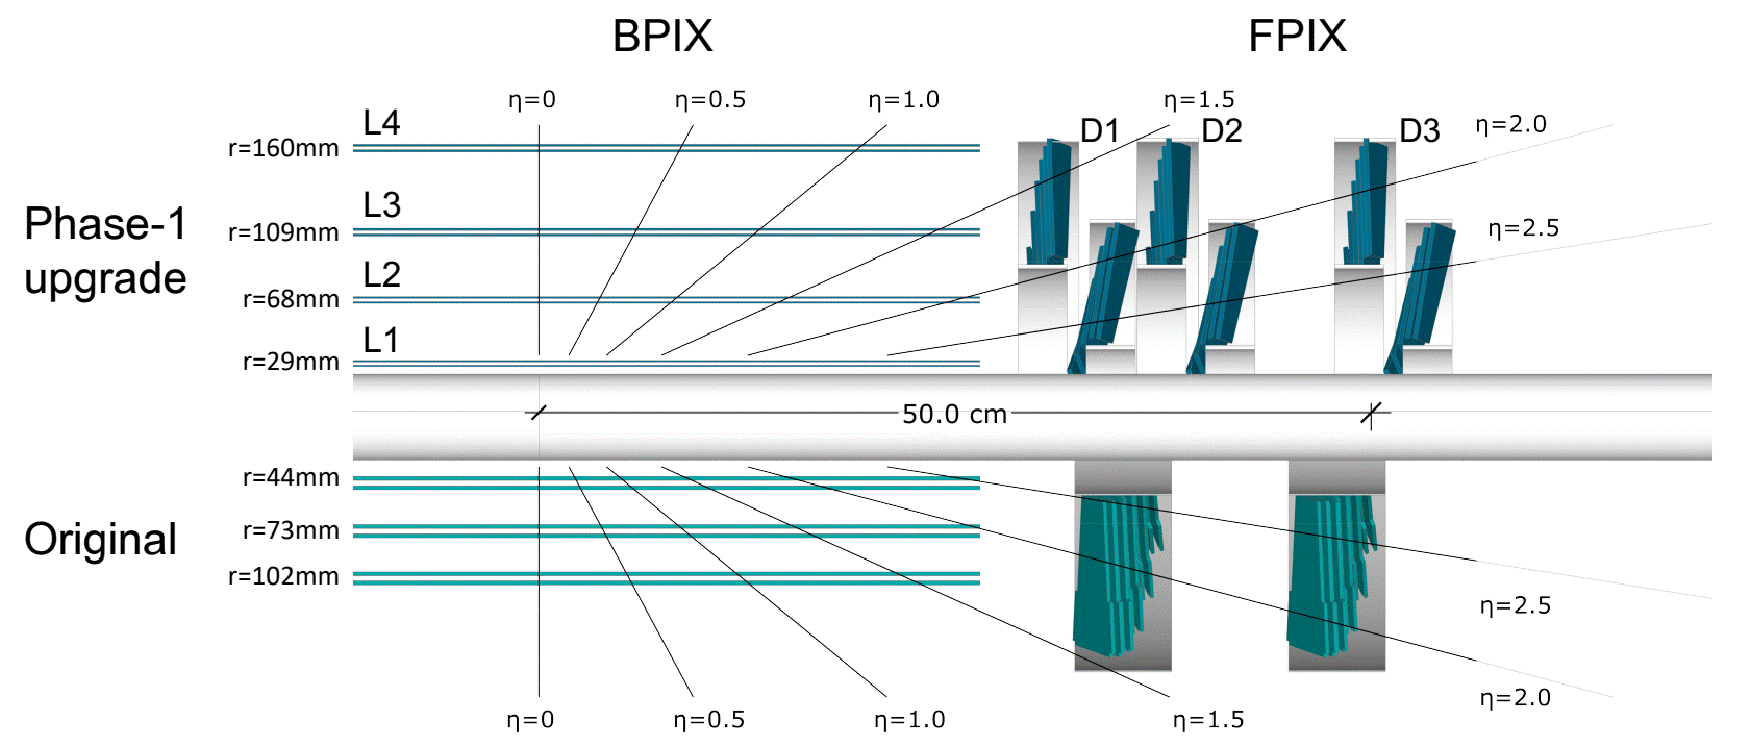
\includegraphics[width=1\textwidth]{Figures/Chapter3/CMS_Pixel_Upgrade.pdf}
\caption[Longitudinal view of CMS pixel detector before and after Phase-1 Upgrade]{Longitudinal view of \ac{CMS} pixel detector comparing its structure before (lower part) and after (upper part) the Phase-1 Upgrade. Figure taken from Ref.~\cite{CMS_Detector_Run3}.}
\label{Figure:Chapter3_Pixel_Upgrade}
\end{figure}

The improved granularity and four-hit coverage introduced in the Phase-1 pixel detector enable robust three-dimensional reconstruction of charged particle trajectories, which is essential for precise identification of both primary and secondary vertices. Consequently, these tracking enhancements lead to improved vertex reconstruction performance. As shown in Fig.~\ref{Figure:Chapter3_Pixel_Vertex_Resolution}, the transverse ($x,y$) vertex resolution achieved with the Phase-1 detector is significantly better than that of the Phase-0 detector.

\begin{figure}[!htbp]
    \centering
    % First row
    \begin{subfigure}[b]{0.49\textwidth}
        \centering
        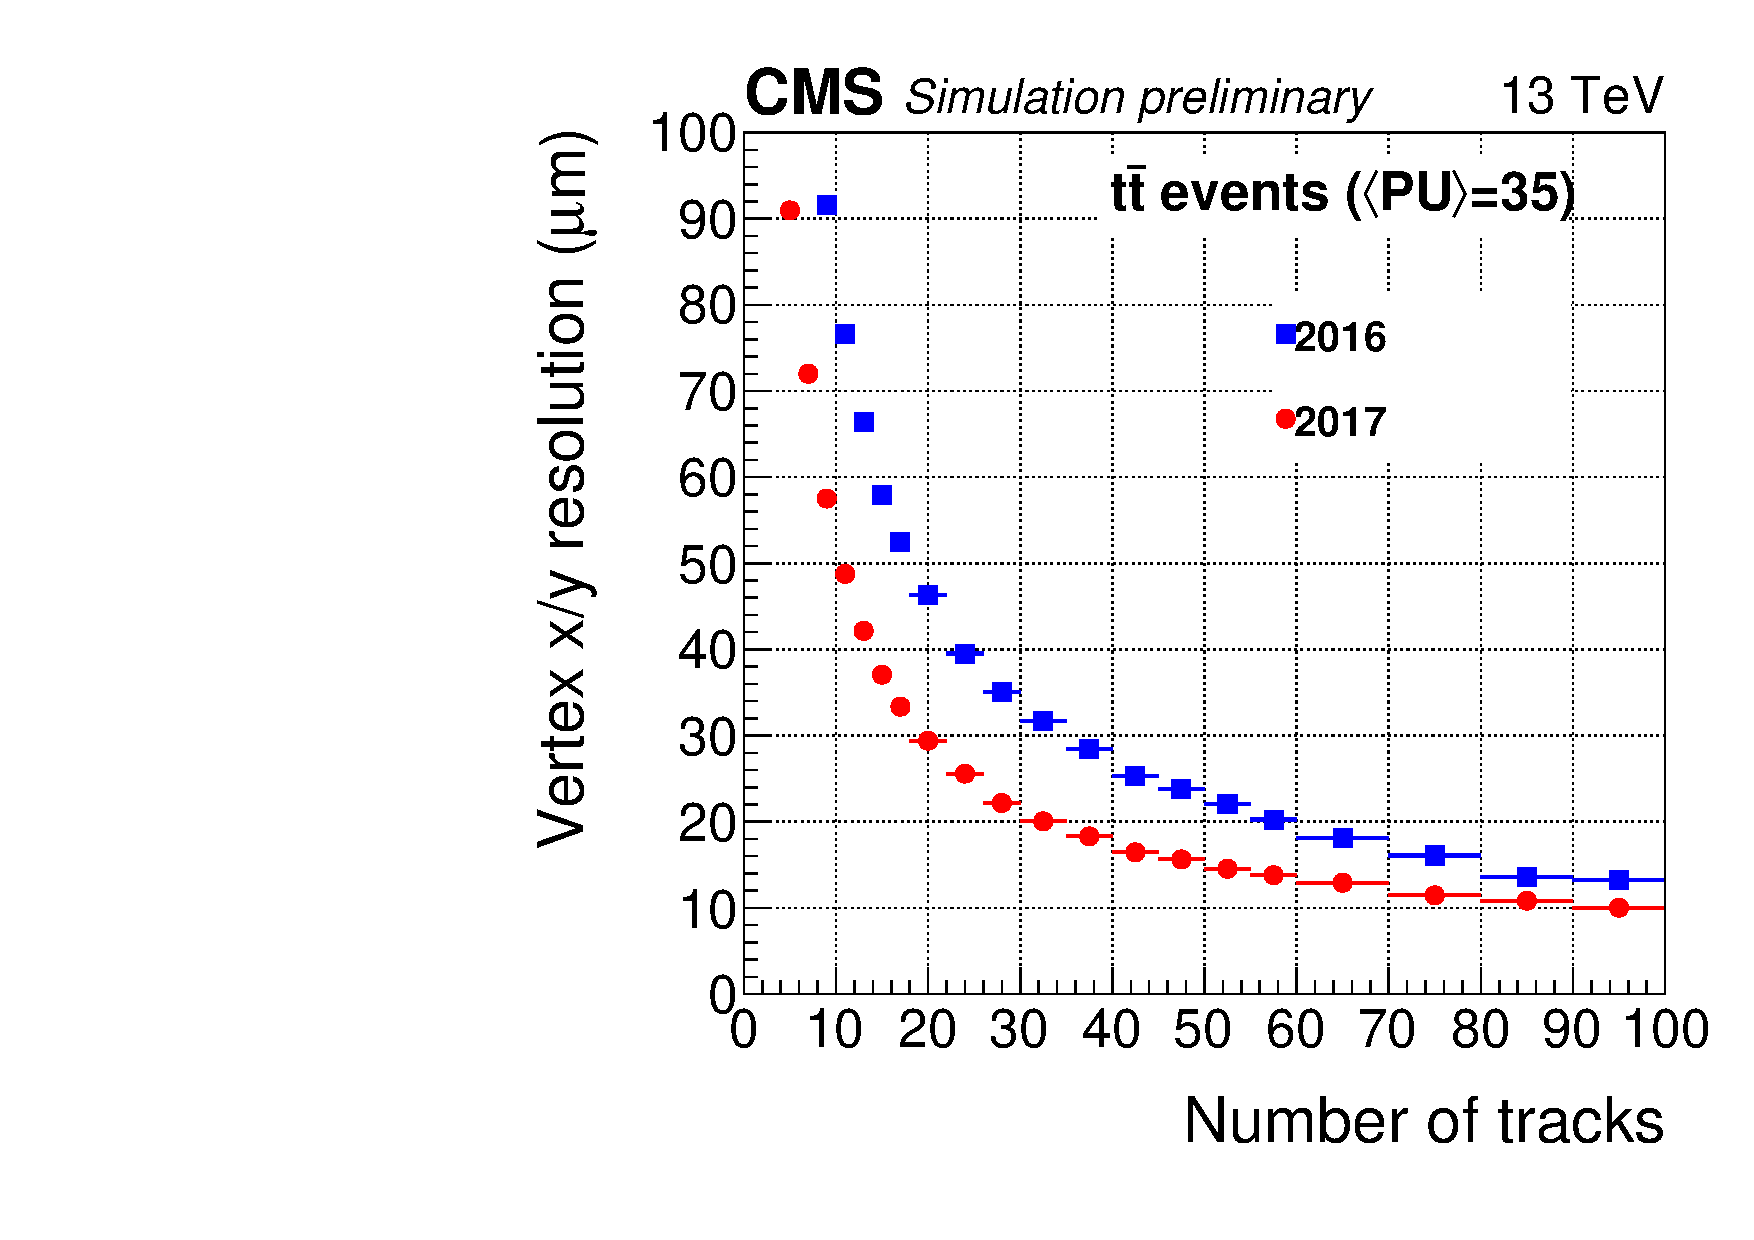
\includegraphics[width=\textwidth]{Figures/Chapter3/Pixel_Vertex_XY_Resolution.pdf}
        \caption{}
    \end{subfigure}
    \begin{subfigure}[b]{0.49\textwidth}
        \centering
        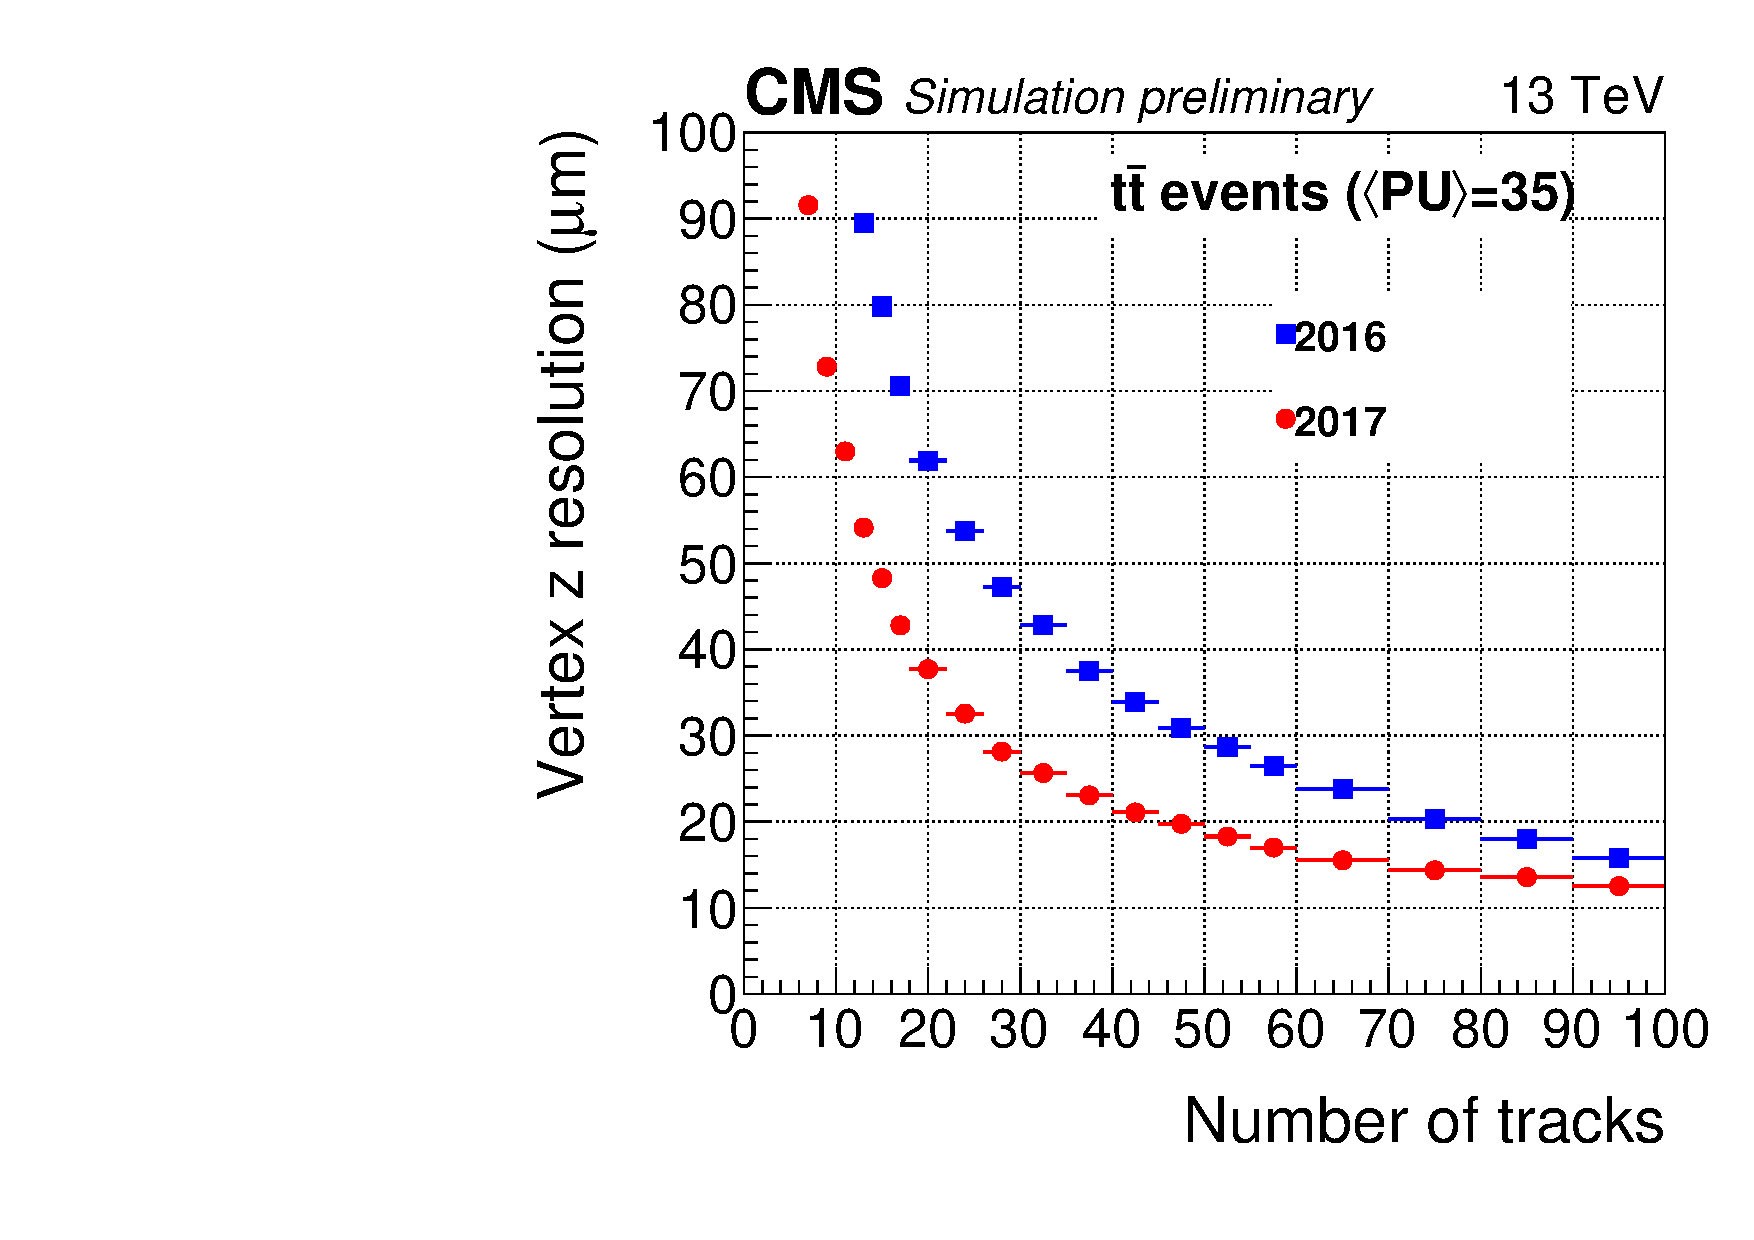
\includegraphics[width=\textwidth]{Figures/Chapter3/Pixel_Vertex_Z_Resolution.pdf}
        \caption{}
    \end{subfigure}
\caption[Vertex resolution comparison between Phase-0 and Phase-1 pixel detectors]{Comparison of the simulated \ac{CMS} vertex resolution between the Phase-0 (blue) and Phase-1 (red) pixel detectors as a function of the number of tracks used in the vertex fit. \textbf{(a)} Transverse ($x,y$) vertex resolution. \textbf{(b)} Longitudinal ($z$) vertex resolution. Figures taken from Ref.~\cite{Pixel_Vertex_Performance}.}

\label{Figure:Chapter3_Pixel_Vertex_Resolution}
\end{figure}


\subsubsection{Silicon Strip Tracker}
Surrounding the pixel detector is the \textbf{\ac{SST}}, illustrated in Fig.~\ref{Figure:Chapter3_Tracker_Geometry}. In the outer tracking region, lower particle occupancy allows the use of silicon strips instead of pixels, relaxing granularity requirements and enabling larger sensor elements. The \ac{SST} covers an active area of approximately $198\unit{m}^2$ and contains 9.3 million silicon micro-strips distributed across 15,148 detector modules. It is composed of four main subsystems: the \ac{TIB}, \ac{TID}, \ac{TOB}, and \ac{TEC}.

\begin{figure}[!htbp]
\centering
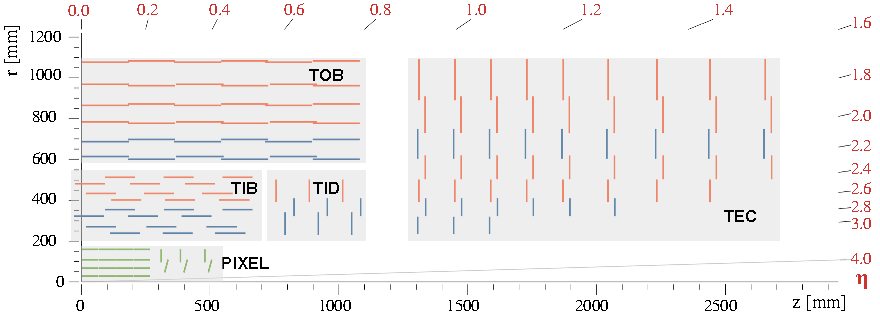
\includegraphics[width=1\textwidth]{Figures/Chapter3/Phase1_Tracker.pdf}
\caption[Schematic of CMS inner tracking system in the ($r$-$z$) plane]{Schematic view of one-quarter of the \ac{CMS} inner tracking system in the ($r$-$z$) plane. The pixel detector is depicted in green, located close to the beamline. Single-sided and double-sided strip modules are depicted as red and blue segments, respectively. Figure adjusted from Ref.~\cite{CMS_Detector_Run3}.}
\label{Figure:Chapter3_Tracker_Geometry}
\end{figure}

The \textbf{\ac{TIB}} is made up of four cylindrical barrel layers located just outside the pixel detector. It provides precise tracking in the central pseudorapidity region and extends out to a radius of $r < 550\unit{mm}$. The strip pitch in the \ac{TIB} ranges from approximately $80-120\unit{\mu m}$, depending on the layer and module type. To ensure complete coverage and continuity in tracking performance, the \ac{TIB} is complemented by the \textbf{\ac{TID}}, which consists of three disk-shaped structures at each end of the \ac{TIB}, extending the longitudinal reach to $|z| < 1180\unit{mm}$. The \ac{TID} uses similar strip pitches, typically around $100-141\unit{\mu m}$. Together, the \ac{TIB} and \ac{TID} form the inner part of the strip tracking system, which is crucial for linking tracks from the pixel detector to the outer layers.

The \textbf{\ac{TOB}} extends the radial coverage beyond the inner systems, occupying the region $r > 550\unit{mm}$. It consists of six cylindrical barrel layers, providing high-precision measurements over a larger area with longer strip modules. The strip pitch in the \ac{TOB} is coarser than in the inner systems, with a pitch of approximately $183\unit{\mu m}$ in the inner \ac{TOB} layers and $122\unit{\mu m}$ in the outer layers. The \ac{TOB} ensures efficient momentum resolution and track reconstruction for particles passing through the outer barrel region, especially those with lower transverse momentum.

The \textbf{\ac{TEC}} completes the strip tracker by covering the forward pseudorapidity regions. Each \ac{TEC} consists of nine disks positioned between $1240 < |z| < 2820\unit{mm}$ on either side of the detector. These disks contain up to seven concentric rings of silicon strip modules, which are carefully arranged to maintain uniform tracking performance and coverage up to $|\eta| \simeq 2.5$. The strip pitch in the \ac{TEC} varies across the radial zones of the disks and generally ranges from $97-184\unit{\mu m}$.

In the barrel sections, the modules are oriented to measure the radial $r\text{-}\phi$ coordinates. Conversely, in the \ac{TID} and \ac{TEC} sections, they are primarily aligned to measure $\phi\text{-}z$ coordinates. The strip pitch varies across layers, giving single point hit resolutions of about 23–35$\unit{\mu m}$ in the TIB, 35–53$\unit{\mu m}$ in the TOB, and a pitch-dependent resolution in the TID and TEC.

In the innermost two layers of the \ac{TIB} and \ac{TOB}, the first two rings of the \ac{TID}, and rings 1, 2, and 5 of the \ac{TEC}, double-sided modules are deployed. These consist of two single-sided sensors mounted back-to-back with a stereo angle of $100\unit{mrad}$. The combination of their signals enables three-dimensional hit reconstruction, providing an additional measurement of the $z$ coordinate in the barrel and the $r$ coordinate in the disk regions.

\subsection{Electromagnetic calorimeter}

As outlined by the \ac{LHC} physics requirements in Section~\ref{Section:Chapter3_CMS_Detector_Introduction}, precise reconstruction of electromagnetic particles and robust suppression of background processes ($\pi^0 \to \gamma \gamma$) are essential for \ac{CMS}. The \ac{CMS} \textbf{\ac{ECAL}}~\cite{LHC_CMS,CMS_Detector_Run3,CMS_ECAL_Performance_Run2} is designed to meet these demands, providing high-resolution energy measurements for electrons and photons. It is composed of three main subsystems: a central barrel calorimeter, two endcap calorimeters, and a preshower detector situated in front of the endcaps.

The \ac{ECAL} is a hermetic homogeneous calorimeter consisting of 61,200 lead tungstate (PbWO$_4$) crystals mounted in the central \textbf{barrel} part. These crystals are arranged in a quasi-projective geometry, with their axes slightly tilted ($3^\circ$) relative to the line from the nominal interaction point. This geometry minimises gaps in the detector and reduces the probability of particles passing through the cracks between crystals. The barrel region covers the pseudorapidity range $|\eta| < 1.479$ and features a 360-fold segmentation in $\phi$ and a ($2 \times 85$)-fold segmentation in $\eta$. Each barrel crystal has a front face cross-section of $22 \times 22\unit{mm}^2$ and a length corresponding to $25.8~X_0$ (radiation lengths), ensuring that most electromagnetic showers are well-contained within a few crystals.

The \textbf{endcap} region complements the barrel coverage, extending the \ac{ECAL} acceptance to $1.479 < |\eta| < 3.0$ with 7,324 crystals in each of the two endcaps. These crystals are larger in cross-section ($28.62 \times 28.62\unit{mm}^2$) and slightly shorter in length compared to those in the barrel, corresponding to $24.7~X_0$. As in the barrel, the PbWO$_4$ crystals are precisely arranged to maintain fine granularity.

The \textbf{Preshower} system is installed in front of the endcaps, covering a fiducial region of $1.653 < |\eta| < 2.6$. It is designed explicitly for $\pi^0$ rejection by distinguishing between closely spaced photon pairs from $\pi^0 \to \gamma \gamma$ decays. The Preshower is a $20\unit{cm}$ ($3~X_0$) thick sampling calorimeter composed of two alternating layers of lead to initiate electromagnetic showers and silicon strip sensors to measure the deposited energy and transverse shower profiles.

The selection of PbWO$_4$ crystals for all \ac{ECAL} regions is motivated by their desirable properties: high density ($8.28\unit{gcm}^{-3}$), short radiation length ($0.89\unit{cm}$), and small Moli\`ere radius ($2.2\unit{cm}$). This allows for a compact and granular calorimeter design. Additionally, these crystals emit about 80\% of their scintillation light within $25\unit{ns}$, matching the \ac{LHC} bunch crossing time and enabling efficient energy collection within a single event window.

A crucial component of the \ac{CMS} \ac{ECAL} is the photodetectors, which convert the scintillation light produced in the PbWO$_4$ crystals into electrical signals. Due to the relatively low light yield of these crystals, the photodetectors must provide internal amplification. They must also exhibit a fast response, high radiation tolerance, and compatibility with the strong longitudinal magnetic field of the \ac{CMS} solenoid ($4\unit{T}$). \textit{\acp{APD})} and \textit{\ac{VPT}} are employed in the barrel and endcap regions, respectively. Although \acp{VPT} offer lower quantum efficiency and gain compared to \acp{APD}, their exceptional radiation hardness and ability to operate in high-field environments make them well-suited for the endcap configuration.

As shown in Figures~\ref{Figure:Chapter3_CMS_schematic}-\ref{Figure:Chapter3_CMS_slice}, the \ac{ECAL} is positioned outside the inner tracking system and in front of the hadronic calorimeter. A schematic of the \ac{CMS} \ac{ECAL} is shown in Fig.~\ref{Figure:Chapter3_CMS_ECAL}.

\begin{figure}[!htbp]
\centering
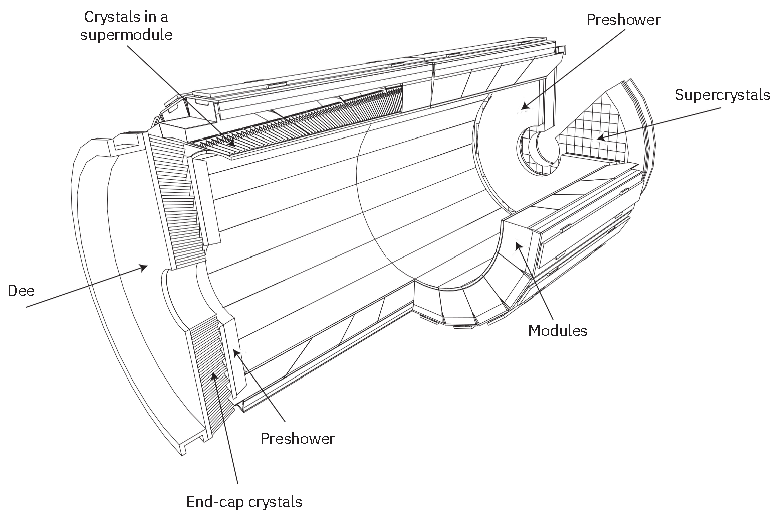
\includegraphics[width= .85\textwidth]{Figures/Chapter3/CMS_ECAL.pdf}
\caption[Schematic view of the CMS Electromagnetic Calorimeter subdetector]{Schematic view of the \ac{CMS} \ac{ECAL} subdetector. Figure taken from Ref.~\cite{LHC_CMS}.}
\label{Figure:Chapter3_CMS_ECAL}
\end{figure}
\newpage
The energy resolution of the \ac{ECAL} is parametrised as a function of the incident particle energy $E$ as:

\begin{equation_pad}
    \left(\frac{\sigma}{E}\right)^2 =  \underbrace{\left(\frac{S}{\sqrt{E}}\right)^2}_{\text{Stochastic}} +  \underbrace{\left(\frac{N}{E}\right)^2}_{\text{Noise}} +  \underbrace{C^2}_{\text{Constant}}
\end{equation_pad}

Each term reflects a different contribution to the resolution: the stochastic term accounts for statistical fluctuations in lateral shower containment and photon yield; the noise term reflects electronic noise and \ac{PU}; and the constant term arises from detector non-uniformities ($\eg$ longitudinal response) and calibration uncertainties. During an electron test beam in 2014~\cite{ECAL_TestBeam}, the \ac{ECAL} demonstrated excellent energy resolution, consistent with the design specifications:

\begin{equation_pad}
    \left(\frac{\sigma}{E}\right)^2 =  \underbrace{\left(\frac{2.8\%}{\sqrt{E}}\right)^2}_{\text{Stochastic}} +  \underbrace{\left(\frac{0.12}{E}\right)^2}_{\text{Noise}} +  \underbrace{(0.30\%)^2}_{\text{Constant}}
\end{equation_pad}

\subsection{Hadronic calorimeter}
To complete the calorimetric measurement and ensure accurate reconstruction of hadronic jets and \ac{MET}, the \ac{CMS} detector employs a dedicated \ac{HCAL} system. Positioned outside the \ac{ECAL}, the \ac{HCAL} is a sampling calorimeter designed to detect strongly interacting particles and spans the pseudorapidity range $|\eta| < 5.2$~\cite{LHC_CMS,CMS_Detector_Run3}. The \ac{HCAL} comprises four distinct components: the \ac{HB}, \ac{HE}, \ac{HO}, and \ac{HF} calorimeters, as shown in Fig.~\ref{Figure:Chapter3_CMS_HCAL}.

\begin{figure}[!htbp]
\centering
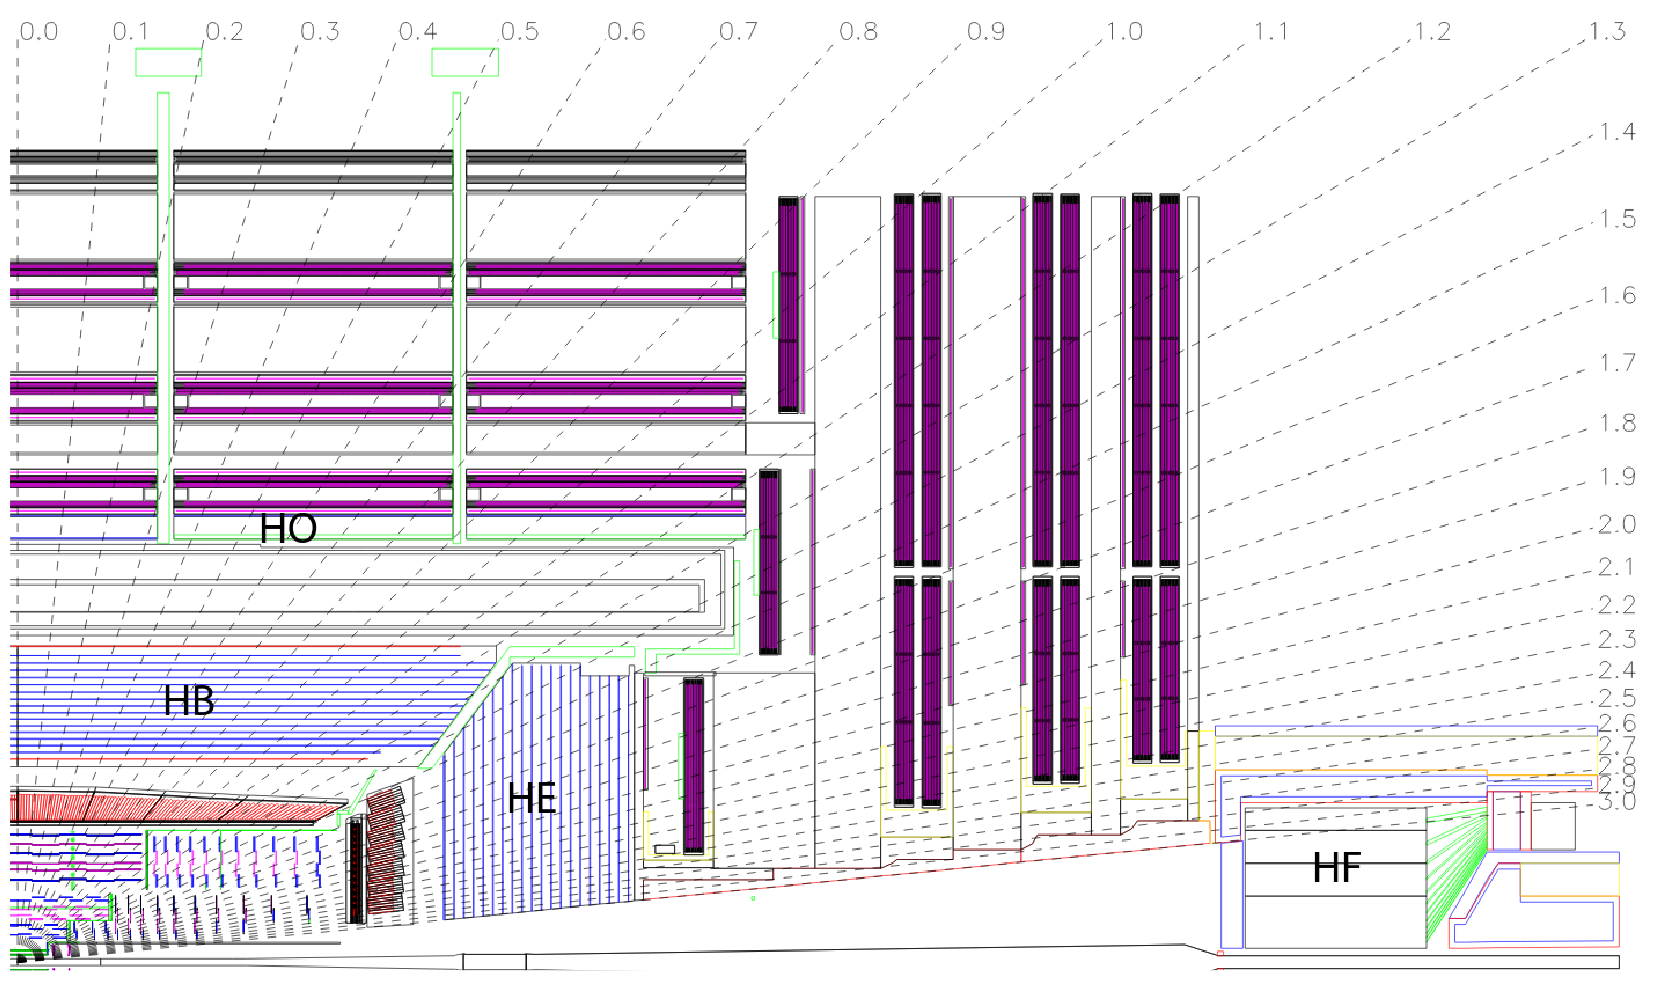
\includegraphics[width= 1.0\textwidth]{Figures/Chapter3/CMS_HCAL.pdf}
\caption[Schematic of CMS detector highlighting Hadronic Calorimeter sub-detectors]{A schematic view of one-quarter of the \ac{CMS} detector with the locations of the \ac{HB}, \ac{HO}, \ac{HE} and \ac{HF} sub-detectors of the \ac{HCAL} being shown. Figure adjusted from Ref.~\cite{LHC_CMS}.}
\label{Figure:Chapter3_CMS_HCAL}
\end{figure}

The \textbf{\ac{HB}} and \textbf{\ac{HE}} subdetectors are located within the bore of the magnet, covering the pseudorapidity regions $|\eta| < 1.3$ and $1.3 < |\eta| < 3.0$, respectively. They are constructed using alternating layers of brass absorber plates and plastic scintillators. Brass is used due to its short nuclear interaction length and non-magnetic nature, the latter being essential for operation within the \ac{CMS} solenoid. The \textbf{\ac{HB}} has a minimum absorber thickness of 5.82 interaction lengths ($\lambda_0$), which increases with polar angle as ($1/\sin\theta$) to approximately 10.6~$\lambda_0$ at $|\eta| = 1.3$. In the \textbf{\ac{HE}}, 79$\unit{mm}$ thick brass plates interleaved with 9$\unit{mm}$ scintillator gaps provide a total depth of around 10~$\lambda_0$, including the contribution from the electromagnetic crystals in front. The calorimeter segmentation is $\Delta\eta \times \Delta\phi = 0.087 \times 0.087$ for $|\eta| < 1.6$, and approximately $0.17 \times 0.17$ for $|\eta| \geq 1.6$. Charged particles from hadronic showers deposit energy in the scintillator tiles, producing scintillation light that is collected by wavelength-shifting fibres and read out using hybrid photodiodes.

Due to the solenoid magnet, the \ac{HB} is radially restricted, constraining the total amount of material which can be inserted to absorb hadronic showers. As a result, the combined stopping power of the EB and \ac{HB} does not provide sufficient containment of the hadronic showers. The \textbf{\ac{HO}} subdetector is used as a tail catcher outside of the solenoid, aiming to ensure adequate sampling depth for $|\eta| < 1.3$. The \ac{HO} employs the same active scintillator as the \ac{HB}, while also utilising the solenoid as an additional absorber, extending the minimum depth to 11.8~$\lambda_0$. This extended sampling is crucial for identifying and measuring the energy of late-starting or highly penetrating showers.

Beyond $|\eta| < 3.0$, the \textbf{\ac{HF}} sub-detector extends the pseudorapidity coverage of the \ac{CMS} \ac{HCAL} to $|\eta| < 5.2$, and is located at $\pm 11.2\unit{m}$ from the interaction point. Its design posed significant challenges due to the extremely harsh radiation environment in the forward region, where particle fluxes reach unprecedented levels. To ensure long-term durability, the \ac{HF} was constructed using highly radiation-resistant materials. Quartz fibres were chosen as the active medium, embedded within a steel absorber composed of 5$\unit{mm}$ thick grooved plates into which the fibres are inserted. The \ac{HF} subdetector is segmented longitudinally into two readout depths: one set of fibres spans the entire 165$\unit{cm}$ depth of the absorber (approximately 10~$\lambda_0$), while the other begins at a depth of 22$\unit{cm}$. By reading out these fibre sets independently, the \ac{HF} can discriminate between electromagnetic showers, which deposit a large fraction of their energy in the first $22\unit{cm}$ and hadronic showers, which deposit their energy more uniformly across the full depth. When charged particles pass through the quartz fibres, they produce Cherenkov light, which is then collected and transmitted to photomultiplier tubes. The use of Cherenkov light makes the \ac{HF} relatively insensitive to low-energy particles and neutral backgrounds, such as neutrons or secondary products from activated radionuclides, helping to reduce noise in this high-radiation environment.

When combining information from the inner tracking system with measurements from the calorimeters, the jet energy resolution typically reaches 15\% at $10\unit{GeV}$, 8\% at $100\unit{GeV}$, and 4\% at $1\unit{TeV}$. In comparison, using only the \ac{ECAL} and \ac{HCAL} calorimeters yields resolutions of approximately 40\%, 12\%, and 5\% at the same energies, respectively~\cite{CMS_HCAL_EnergyResolution}.

\subsection{Muon system}
To satisfy the \ac{LHC}’s stringent performance goals for muon reconstruction, \ac{CMS} employs a dedicated muon tracking system~\cite{LHC_CMS,CMS_Muon_System_Performance} positioned furthest from the interaction point. The system serves three primary functions: muon identification, momentum measurement, and triggering. These are made possible by the strong solenoidal magnetic field and the iron return yoke, which acts as a hadron absorber.  \ac{CMS} employs three complementary gaseous particle detector technologies for detecting muons.  

In the barrel region, where muon rates and neutron-induced backgrounds are relatively low, the $3.8\unit{T}$ magnetic field is uniform and largely confined within the iron yoke. \textbf{\acp{DT}} are used here, providing coverage in the pseudorapidity region $|\eta| < 1.2$. These are organised into four stations interspersed among the layers of the flux return plates. The first three stations are further subdivided into eight chambers, four measuring the muon coordinate in the $r$-$\phi$ bending plane and four providing a measurement in the $z$ direction. Conversely, the capabilities of the fourth muon station are restricted to $r$–$\phi$ measurements. Each \ac{DT} chamber consists of rectangular drift cells containing a central anode wire. The cells are filled with a gas mixture of argon and carbon dioxide, which enables efficient ionisation and drift of electrons toward the wire for signal detection. 

In contrast to the barrel region, the endcaps are subjected to higher muon rates and background levels. The magnetic field in this region is both strong and non-uniform, necessitating a finely segmented detector system that is radiation-resistant and capable of fast response times. To meet these demands, \ac{CMS} employs \textbf{\acp{CSC}} in the region $0.9 < |\eta|<2.4$. Each \ac{CSC} is a multi-layered gaseous detector consisting of six planes of anode wires interleaved with seven cathode layers. In both endcaps, the chambers are arranged into four stations placed perpendicular to the beam line and embedded between the layers of the iron yoke. The cathode strips extend radially outward from the beam axis, providing precise position measurements in the $r$-$\phi$ plane. The anode wires, oriented roughly perpendicular to the strips, deliver additional spatial information in $\eta$ and enable timing measurements relative to the beam crossing. This six-layer configuration enhances pattern recognition, improving the rejection of spurious hits from background sources and allowing for efficient correlation with hits from other stations and with tracks reconstructed in the inner tracker.

The \ac{DT} and \ac{CSC} systems are complemented by the \textbf{\ac{RPC}} system in the pseudorapidity region $|\eta| < 1.6$. RPCs are double-gap chambers featuring anode and cathode plates separated by gas. Compared to \acp{DT} and \acp{CSC}, \acp{RPC} exhibit lower granularity; however, they offer a faster response and good time resolution. These characteristics make them particularly well-suited for use as trigger detectors. As such, they are especially valuable in scenarios where the \ac{DT} and \ac{CSC} systems may struggle to cope with \ac{PU}-induced background. Additionally, RPCs contribute to resolving ambiguities when reconstructing tracks from multiple hits within a chamber, further enhancing the overall performance of the muon detection system.

A schematic illustration of the \ac{CMS} muon detection system is shown in Fig.~\ref{Figure:Chapter3_CMS_Muon_System}, highlighting the arrangement of the \ac{DT}, \ac{CSC}, and \ac{RPC} subdetectors within the return yoke. Owing to its design, the \ac{CMS} muon system achieves a reconstruction and identification efficiency exceeding 95\% for muons with energies above a few GeV. The momentum resolution varies between 1\% and 6\% for transverse momenta below $100\unit{GeV}$, and remains better than 10\% up to $1\unit{TeV}$~\cite{CMS_Muon_System_Performance_2}. Furthermore, the system reliably determines the muon charge sign for transverse momenta up to $1\unit{TeV}$.


\begin{figure}[!htbp]
\centering
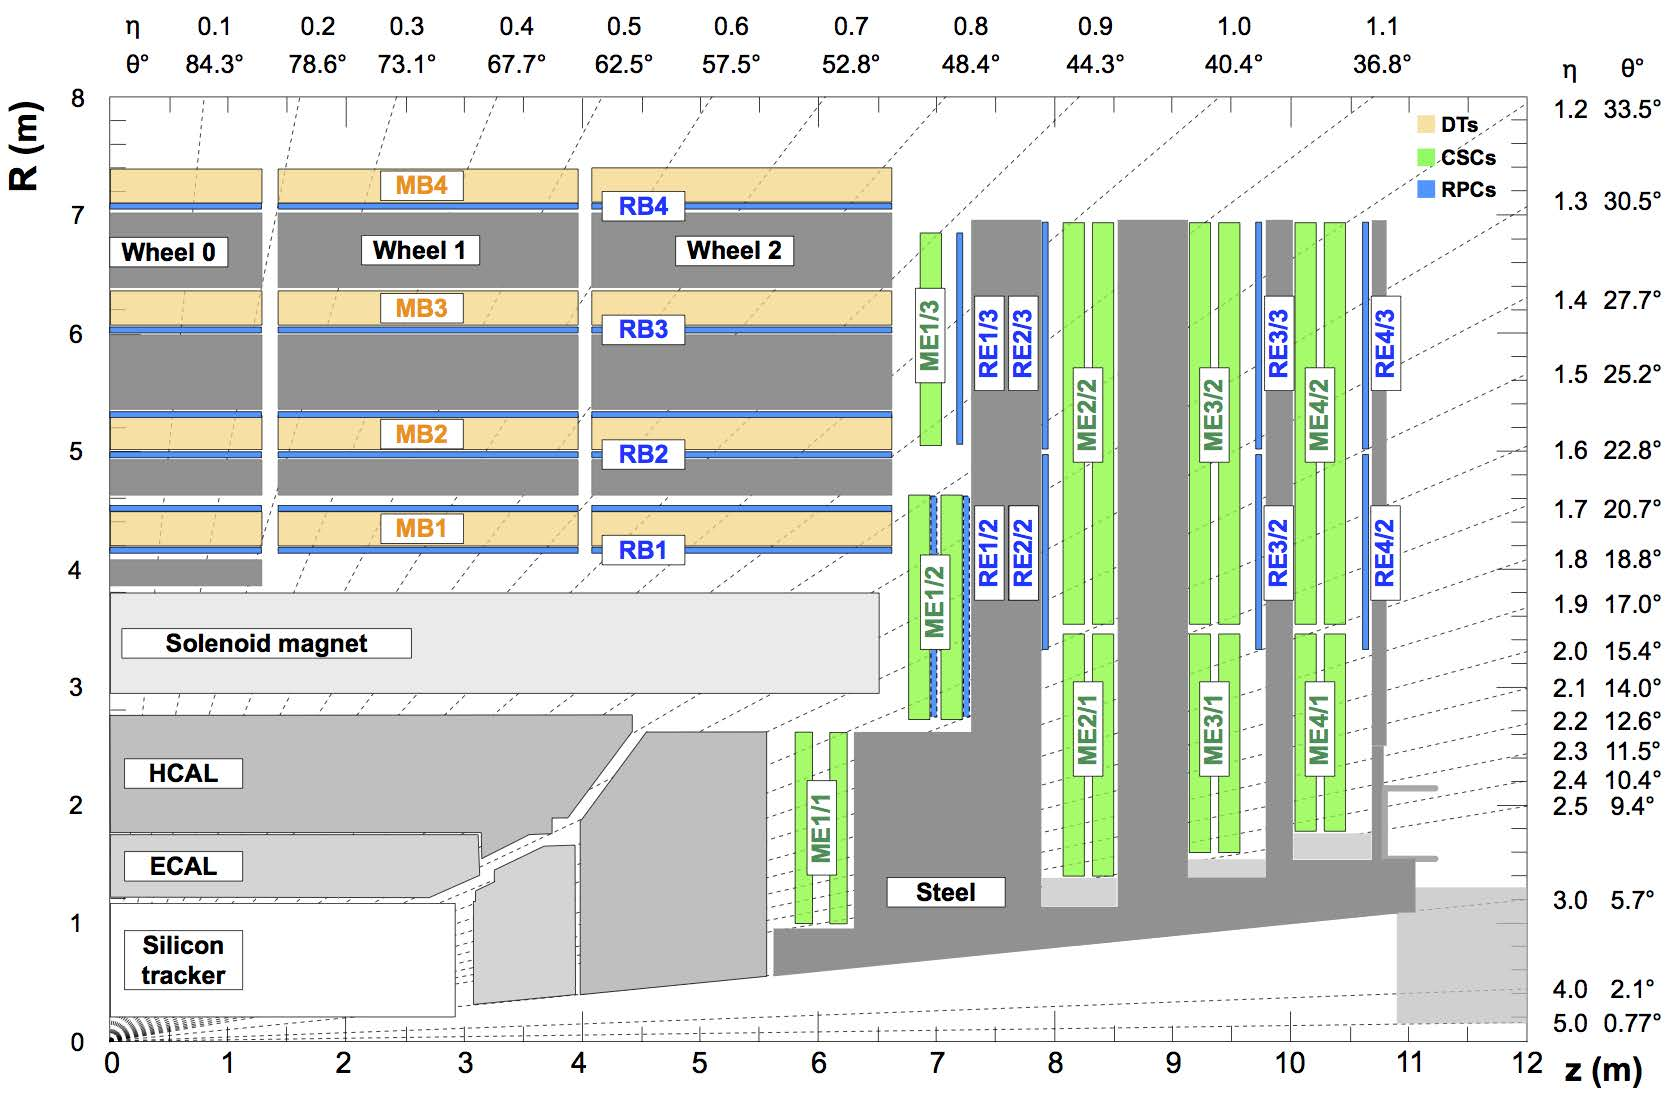
\includegraphics[width= 1.0\textwidth]{Figures/Chapter3/CMS_Muon_System.pdf}
\caption[Schematic of CMS muon detection system]{Schematic illustration of one quarter of the \ac{CMS} detector, highlighting the muon detection system. The \ac{DT} stations are labelled as MB (Muon Barrel), while the \acp{CSC} are labelled as ME (Muon Endcap). The RPCs are denoted as RB in the barrel region and RE in the endcap region. Figure taken from Ref.~\cite{CMS_Muon_System_Performance}.}
\label{Figure:Chapter3_CMS_Muon_System}
\end{figure}

\subsection{Trigger system}

At the \ac{LHC} interaction points, proton bunches cross every $25\unit{ns}$, resulting in a nominal bunch crossing frequency of $40\unit{MHz}$. Additionally, each bunch crossing can yield up to more than 50~\ac{PU} interactions corresponding to an aggregate rate of individual proton-proton interactions surpassing $1\unit{GHz}$. Recording all of these collisions is not feasible nor necessary, as only a small fraction contains events of interest to the \ac{CMS} physics programme. To select the most interesting events, \ac{CMS} employs a dedicated two-level trigger system~\cite{CMS_Trigger} consisting of the \textbf{\ac{L1} trigger} and the \textbf{\ac{HLT}}.

As the name suggests, the \textbf{\ac{L1} trigger} is the first level of the \ac{CMS} trigger system, implemented as a hardware-based trigger on custom-built Field Programmable Gate Arrays with a fixed latency of $4\unit{\mu s}$. \ac{CMS} relies on this system to rapidly determine whether an event should be tentatively accepted or rejected based on calorimeter energy deposits and muon detector hits. The \ac{L1} decision chain comprises three primary subsystems: the \ac{L1} calorimeter system, the \ac{L1} muon trigger system and the global trigger (GT), as shown in Fig.~\ref{Figure:Chapter3_CMS_L1_Trigger}.

\begin{figure}[!htbp]
\centering
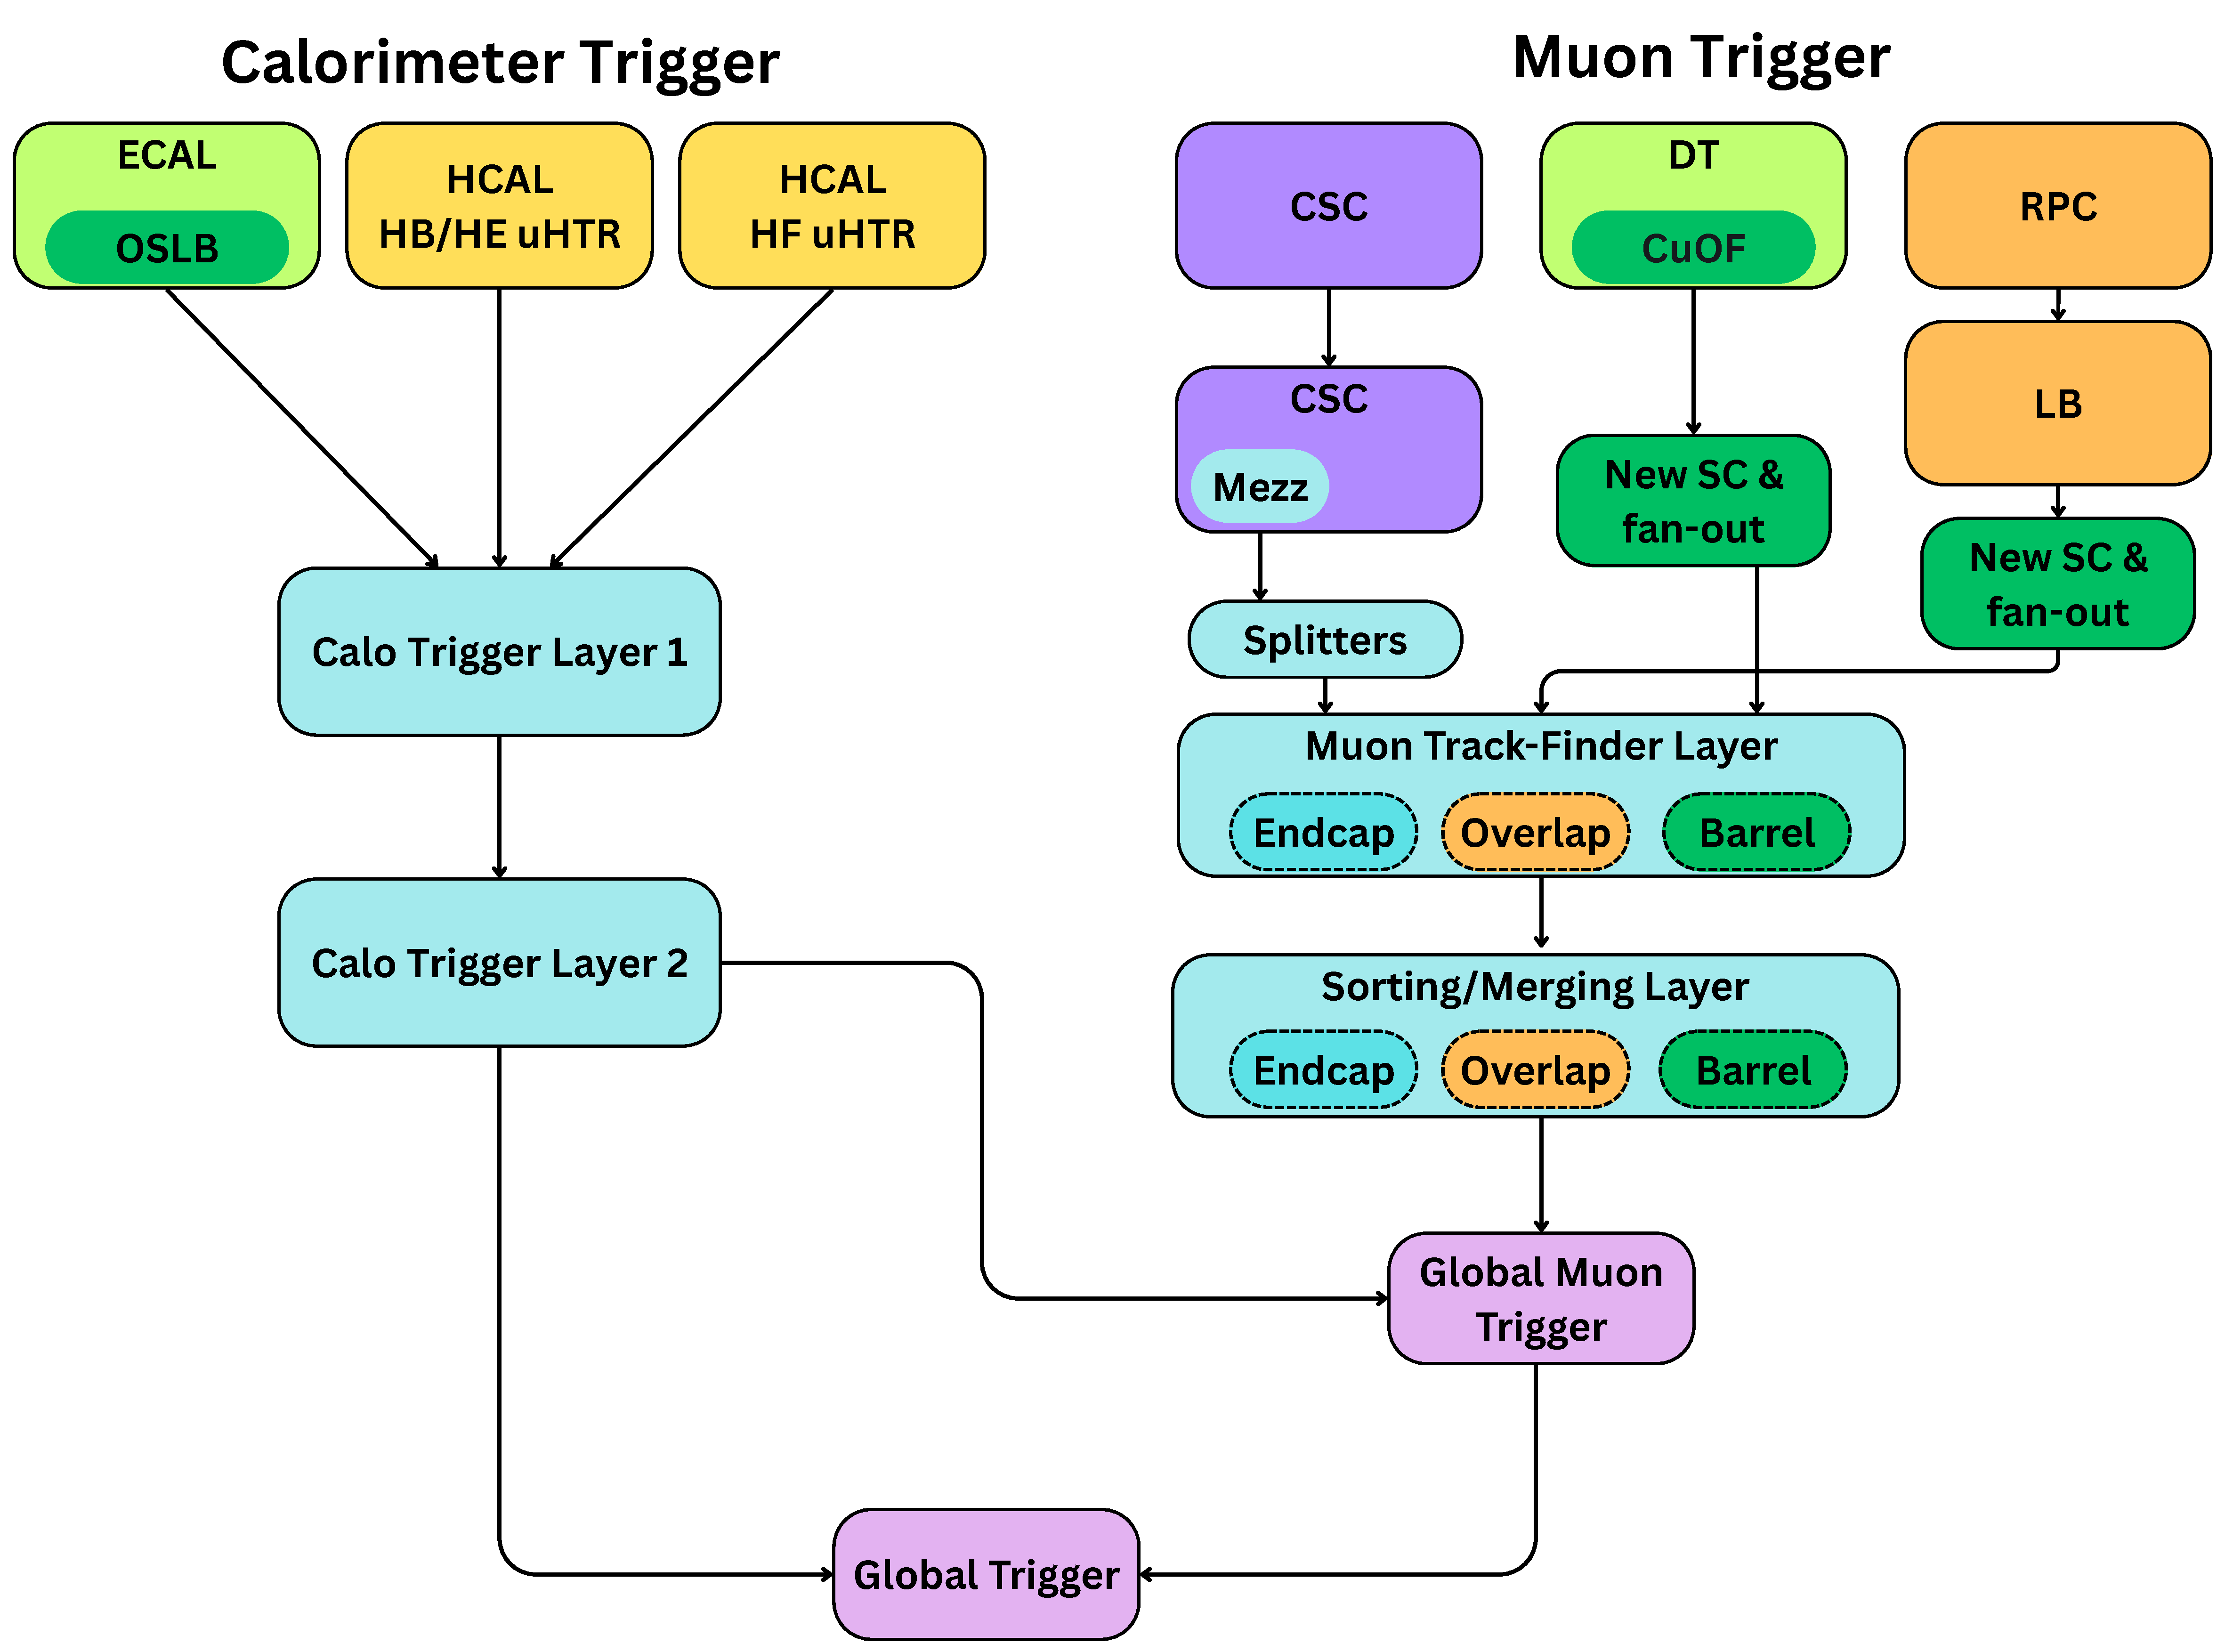
\includegraphics[width= 1.0\textwidth]{Figures/Chapter3/CMS_L1_Trigger.pdf}
\caption[Schematic of the CMS Level-1 trigger workflow]{Schematic of the \ac{CMS} \ac{L1} trigger workflow. Figure reproduced from Ref.~\cite{CMS_L1_Trigger}.}
\label{Figure:Chapter3_CMS_L1_Trigger}
\end{figure}

The \textbf{\ac{L1} calorimeter trigger system} is organised into two processing layers. Layer-1 (\textit{Calo Trigger Layer 1}) receives trigger primitives (energy deposits) from the \ac{ECAL} and the \ac{HCAL}, performs initial calibrations, and sorts local energy deposits. Layer-2 (\textit{Calo Trigger Layer 2}) processes the calibrated information to reconstruct and further calibrate high-level physics objects such as electrons, photons, jets, taus, and \ac{MET}. Simultaneously, hits from the three muon subsystems are processed by the first stage of the \textbf{\ac{L1} muon trigger system} (\textit{Muon Tracking-Finder Layer}). At this stage, track finding is performed by combining hits within sectors in $\phi$ and $\eta$. The reconstructed track candidates are then forwarded to the \textit{Sorting and Merging Layer}, where information from the $\phi$ sectors is consolidated. The output, along with the calorimeter information required to compute isolation, is passed to the global muon trigger, where a sorted list of muon candidates for the entire detector is produced. Finally, the \textbf{global trigger} integrates the information from both the \ac{L1} calorimeter and muon trigger systems, enabling it to make a decision on the fate of the event. This allows for the event rate to be reduced from $40\unit{MHz}$ to $100\unit{kHz}$.

The \textbf{\ac{HLT}} system is the second stage of the \ac{CMS} trigger architecture. It is a software-based trigger that runs on a processor farm composed of commercial CPUs. In contrast to the hardware-based \ac{L1} trigger, the \ac{HLT} utilises full-resolution data from the \ac{CMS} detector and applies offline-quality reconstruction algorithms for more refined event selection. The primary objective of the \ac{HLT} is to further reduce the event rate to about $1\unit{kHz}$ for permanent storage and offline analysis. 

Rather than operating with fixed latency, the \ac{HLT} processes events asynchronously, scaling with available CPU resources. Its workflow is organised into \ac{HLT} paths, each consisting of a predefined sequence of algorithmic steps that reconstruct and select physics objects. These paths are structured to increase in complexity, precision, and physics sophistication. To optimise computational efficiency, initial selections use fast information from the calorimeters and muon detectors, while CPU-intensive tracking is applied only to events that pass these preliminary filters. 

Events accepted by the \ac{HLT} are handed off to the storage manager, which writes them temporarily to local disk. They are then transferred to the \ac{CMS} Tier‑0 computing centre for offline reconstruction and long‑term archival.


